% VANTAGE: Hidden Rewrite Views for Fixed-Prompt Speculative Code-Edit Decoding
% Focused submission draft.

\documentclass[11pt,a4paper]{article}
\usepackage[utf8]{inputenc}
\usepackage[T1]{fontenc}
\usepackage[margin=1in]{geometry}
\usepackage[protrusion=true,expansion=false]{microtype}
\usepackage{booktabs}
\usepackage{xcolor}
\usepackage{amsmath}
\usepackage{listings}
\usepackage{graphicx}
\usepackage{cite}
\usepackage{array}
\usepackage{hyperref}

\newcolumntype{L}[1]{>{\raggedright\arraybackslash}p{#1}}
\setlength{\emergencystretch}{3em}

\hypersetup{
  colorlinks=true,
  linkcolor=blue!50!black,
  citecolor=blue!50!black,
  urlcolor=blue!50!black,
  pdftitle={VANTAGE: Hidden Rewrite Views for Fixed-Prompt Speculative Code-Edit Decoding},
  pdfauthor={Faizan Ahmed},
}

\title{\vspace{-1.0em}\textbf{VANTAGE: Hidden Rewrite Views for Fixed-Prompt Speculative Code-Edit Decoding}}
\author{Faizan Ahmed\\Headstarter\\\texttt{faizan@theheadstarter.com}}
\date{\today}

\begin{document}
\maketitle

\begin{abstract}
Prompt lookup decoding (PLD) is a strong model-free accelerator for
copy-heavy code edits, but literal prompt recurrence breaks near systematic
reference drift. We introduce \textbf{VANTAGE}, a fixed-prompt speculative
decoder whose core primitive, \emph{Rewrite-View Lookup}, materializes
prompt-visible explicit rewrites as an internal draft source while leaving the
target model's visible prompt unchanged. Every emitted draft token is
target-verified, and every correction or bonus token is emitted directly from
target argmax logits. Thus, under an exact deterministic verifier, the hidden
view can affect latency but not the fixed-prompt greedy output; our fp32/eager
and fp32/sdpa audits confirm this on the controlled workloads. On
Qwen2.5-Coder-7B controlled explicit-map Python edit workloads, the audited
fp32/sdpa path is
\textbf{1.28$\times$} faster than tuned PLD on field substitutions,
\textbf{1.64$\times$} faster on identifier-style substitutions, and
\textbf{1.33$\times$} faster on a mixed suite, with PLD and VANTAGE/SafeRoute
both matching vanilla greedy on 100/100 prompts in every audited workload. The
result is a controlled mechanism study: deterministic hidden views can recover
speculative copy opportunities that literal PLD misses while preserving the
original prompt-conditioned greedy behavior. The evidence is limited to
explicit-map, high-copy workloads; bf16 paths still drift, multi-view
real-commit evidence remains preliminary, and we do not claim production
serving, broad edit quality, multi-model universality, or sampling preservation.
\end{abstract}

% -----------------------------------------------------------------------------
\section{Introduction}

Many code-edit prompts are copy-heavy: the requested output preserves most of a
reference program while changing a small number of names, fields, literals, or
local conventions. This makes prompt lookup decoding (PLD) a very strong
baseline. PLD searches the literal prompt and generation history for exact token
recurrence, proposes the following tokens, and verifies them with the target
model. We therefore compare against a tuned BlazEdit-style long-window PLD row,
using it as the literal-copy baseline throughout the primary experiments.

The gap we study is narrower than general code editing. Literal recurrence can
break under systematic edit drift even when the target output remains
structurally aligned to the reference. For example:

\begin{lstlisting}[basicstyle=\ttfamily\tiny,frame=single]
# reference
def get_user_name(user):
    return user.name.strip().lower()

# instruction: rename user to account

# target output
def get_user_name(account):
    return account.name.strip().lower()
\end{lstlisting}

The function name is intentionally unchanged: the rewrite is boundary-aware and
does not rewrite substrings such as \texttt{get\_user}.
PLD can copy the unchanged regions, but recurrence around \texttt{user} and
\texttt{account} is broken. A hidden rewrite view that applies
\texttt{user -> account} to the prompt-visible reference restores a target-side
copy source without changing the prompt seen by the model. We call this
\emph{reference drift}: the target remains aligned to a deterministic
prompt-derived view, while the literal prompt no longer contains the exact
future token span.

VANTAGE is the validated decoder in this paper. Its core primitive,
Rewrite-View Lookup, extracts explicit prompt-visible rewrite maps, materializes
the transformed reference, tokenizes that whole transformed reference, and uses
it only as a speculative draft source. The target model remains the sole
emission authority under the original prompt: draft tokens are emitted only
after target verification, and corrections or bonus tokens are emitted directly
from target argmax logits. In the audited fp32/sdpa controlled validation,
VANTAGE with SafeRoute reduces verifier steps by
44.7--66.3\% on structured explicit-map workloads while routing zero-drift
prompts back to the same exact PLD path.

This is not a claim that explicit lexical rewrite tasks require an LLM. If an
application can bypass the model or visibly rewrite the prompt, a deterministic
rewrite engine or transformed-reference prompt injection may be simpler and
faster. VANTAGE targets the stricter fixed-prompt setting: preserve the target
model's original prompt-conditioned greedy behavior while reducing latency. In
that setting, deterministic prompt-derived code views sit between literal prompt
reuse and neural draft models: they expose high-acceptance draft spans that PLD
cannot see, while leaving draft acceptance, corrections, and bonus emissions to
the target verifier.

\paragraph{Scope.}
The exact-path throughput claim is conditional: it holds on Qwen2.5-Coder-7B
controlled structured Python edit workloads with prompt-visible explicit
rewrite maps. On these workloads, the target verifier often accepts long
rewrite-view spans, which explains the measured speedups. The broader
view-based framework remains preliminary: the real-commit artifact is a
single-run bf16 timing diagnostic with output drift. Some multi-view variants
show small diagnostic speedups while rewrite-view-only loses, but this is not
exact-path validation. The locked controlled
rows are run as fixed manifests rather than filtered after timing, and the
separate exact-target/syntax diagnostics report imperfect task quality and
local rewrite compliance separately. It is not a vLLM production-serving claim,
not a broad real-commit-quality claim, not a multi-model universality claim,
and not a sampling-distribution preservation claim. Instruction-tuned variants
of Qwen and DeepSeek were evaluated only as untemplated sensitivity diagnostics
and do not support a deployment-level instruction-model claim.
Section \ref{sec:boundary} characterizes this instruction-compliance boundary.

\paragraph{Contributions.}
\begin{itemize}
\item We define \textbf{view-based prompt lookup}: PLD is identity-view lookup,
  and a hidden deterministic prompt-derived view may be used as a draft source
  without changing the target model's visible prompt.
\item We introduce \textbf{VANTAGE}, the validated fixed-prompt decoder, and
  its core primitive \textbf{Rewrite-View Lookup}: prompt-visible explicit
  rewrites are materialized into a transformed reference, whole-tokenized,
  indexed, and used only for target-verified draft proposals. SafeRoute routes
  no-map controls back to exact PLD.
\item We state the verifier invariant precisely. Under an exact deterministic
  target oracle, any proposal source used under this verifier and cache-update
  contract preserves fixed-prompt greedy decoding when the decoder emits draft
  tokens only after target verification and emits corrections or bonus tokens
  directly from target argmax logits.
  Implementation audits pass on fp32/eager and fp32/sdpa for the controlled
  workloads, while bf16 remains a diagnostic path with observed drift.
\item We provide controlled evidence on Qwen2.5-Coder-7B explicit-map Python
  edits: VANTAGE/SafeRoute is 1.28--1.64$\times$ faster than tuned PLD on the
  audited fp32/sdpa path, cuts verifier steps by 44.7--66.3\%, and accepts
  91--102 tokens per rewrite-view hit. A same-backend matched-policy
  ablation on structured rows confirms that Rewrite-View Lookup, not only min/max lookup
  flexibility, improves matched-policy identity lookup on structured
  workloads. Preliminary multi-view real-commit rows are reported as
  diagnostics, not as primary evidence.
\end{itemize}

\begin{center}
\fbox{\begin{minipage}{0.93\linewidth}
\textbf{Scope of claims.} This paper evaluates a single-request research
decoder. The primary claim is restricted to VANTAGE/SafeRoute on
Qwen2.5-Coder-7B controlled structured Python edit manifests with
prompt-visible explicit rewrite maps, the tuned
\texttt{blazedit\_pld\_w128\_n10} comparator, deterministic greedy decoding,
audited fp32/sdpa throughput, and fp32/eager/fp32/sdpa exactness audits.
bf16 timing, prompt injection, instruction-model sensitivity, route-margin
rows, and multi-view real-commit rows are diagnostics unless separately
validated on an exact repeated-timing path. The paper does not claim
production-serving superiority, broad real-commit-quality improvement,
multi-model universality, or stochastic sampling preservation.
\end{minipage}}
\end{center}

Appendix Table~\ref{tab:detailed-claim-audit} gives the full
claim-to-evidence ledger.

% -----------------------------------------------------------------------------
\section{Background}

\paragraph{Speculative decoding.}
Speculative decoding drafts candidate tokens from a cheap source and
verifies them with the target model in a batched forward pass
\cite{leviathan2023,chen2023}. In greedy decoding, a draft token is
accepted only if it equals the target argmax at that position; at the
first mismatch, the verifier emits the target correction. Incorrect
drafts can waste time but cannot change the deterministic target-greedy
output when the numerical execution is fixed.

\paragraph{Prompt lookup decoding.}
PLD replaces the neural draft model with exact token reuse. It searches
prior prompt/generated tokens for an exact n-gram occurrence of the
current suffix and proposes the following continuation. This family
includes prompt lookup decoding, n-gram speculation, and suffix-based
model-free speculation \cite{promptlookup,hfpld,vllmngram,tensorrtngram,suffixdecoding}.
In view-based terminology, PLD is \emph{identity-view lookup}: the hidden view
is just the literal prompt/reference/history token pool. We do not claim exact
lookup as novel; PLD is the baseline and primitive that VANTAGE extends through
Rewrite-View Lookup.

We use a BlazEdit-style long-window PLD configuration as the comparator because
preliminary in-harness comparator-selection runs on copy-heavy synthetic
repository edits and CodeEditorBench-style subsets \cite{codeeditorbench} found
it to be the strongest literal-copy baseline among the PLD variants we tried. Those preliminary
comparator-selection runs are not used as quantitative evidence; all reported
claims compare directly against the displayed tuned PLD rows in the primary
exact-path and same-policy artifacts.

\paragraph{Reference drift.}
An edit target exhibits reference drift when most output tokens are
copied or transformed from a reference program, the output remains
aligned to that reference, and exact recurrence is disrupted by a
systematic edit. Table \ref{tab:regimes} summarizes the regimes.

\begin{table}[h]
\centering\scriptsize
\caption{Reference-drift regimes and expected draft behavior.}
\label{tab:regimes}
\resizebox{\linewidth}{!}{%
\begin{tabular}{llll}
\toprule
Regime & Example & PLD & VANTAGE/SR \\
\midrule
Verbatim copy & unchanged output & strongest baseline & route to PLD \\
Explicit drift & rename, field migration, identifier-style substitution & misses near edits & Rewrite-View Lookup \\
Semantic rewrite & new control flow/algorithm & weak & weak/control \\
\bottomrule
\end{tabular}}
\end{table}

% -----------------------------------------------------------------------------
\section{Method}
\label{sec:method}

\subsection{View-based prompt lookup}

View-based prompt lookup generalizes PLD from a single literal token pool to a
set of deterministic hidden prompt-derived code views. A view constructor
$f_i$ maps the visible prompt/reference $P$ to a materialized draft source
\[
  V_i = f_i(P).
\]
The transformed view is never appended to, or exposed as, the visible prompt.
Only selected candidate tokens from the view are passed to the target verifier
as ordinary speculative draft tokens. Rejected draft tokens never become part
of the emitted prefix, and their K/V entries are discarded by the cache-update
rule. Each view is tokenized, indexed, and
queried only by the decoder. A view candidate is a root-excluded continuation
proposed after the current target root token. The target verifier accepts a
matching prefix and emits the target argmax at the first mismatch, exactly as
in greedy speculative decoding.
Thus a bad view can hurt latency, but under exact deterministic verification it
cannot change the fixed-prompt greedy output.

This abstraction makes exact PLD a special case rather than a separate
mechanism: PLD is lookup over the identity view of the prompt/reference. The
validated VANTAGE/SafeRoute instance adds one derived rewrite view that exposes
copyable structure hidden from literal PLD while preserving the same
target-verification contract.

\subsection{Preliminary ViewBank terminology}

The implementation repository also contains preliminary ViewBank variants used
only in diagnostic real-commit timing artifacts. These include patch/frontier,
rescue, cursor, and hunk-local views. They are deterministic prompt-derived
views, but they are not part of the primary exact-path claim and are described
in Appendix \ref{app:viewbank-terminology} for artifact terminology. The
validated VANTAGE/SafeRoute instance uses only the identity PLD view and the
rewrite view built by Rewrite-View Lookup.

\subsection{Rewrite-View Lookup: the rewrite-map view constructor}

Let $R$ be the reference program text and $\phi$ be an explicit rewrite
map extracted from the prompt, such as \texttt{old}$\rightarrow$\texttt{new}.
Exact PLD indexes the identity surface view of the prompt/reference.
Rewrite-View Lookup instead builds a \emph{prompt-defined lookup view}:
\[
  T = \phi(R), \qquad V = \mathrm{tokenize}(T).
\]
The transformed text $T$ is materialized before decoding and tokenized
as a whole. This is important: tokenizer IDs depend on left context for
SentencePiece/BPE tokenizers, so tokenizing a rewritten span in
isolation can produce wrong boundary tokens. The decode loop then uses
the same operation as PLD: exact n-gram lookup over a token index and
target verification of the proposed continuation.

We make this tokenizer-boundary issue explicit in a generated tokenization
audit, with script and output path recorded in the reproducibility appendix.
For Qwen2.5-Coder-7B, transforming
\texttt{~~~~return user.name.strip()} to
\texttt{~~~~return account.name.strip()} gives relevant whole-reference
token IDs \texttt{[470, 2692, 2644, 17181]}, whereas the unsafe
piecemeal construction \texttt{tokenize(prefix) + tokenize(account) +
tokenize(suffix)} gives \texttt{[220, 4608, 2644]}. A
snake-case identifier rewrite similarly differs, while a checked dotted
attribute example does not. The implementation therefore treats
whole-reference tokenization as the default invariant, not an optional
optimization.

\paragraph{Rewrite extraction.}
\texttt{extract\_explicit\_rewrites} is intentionally small and
prompt-only. It extracts explicit pairs in the instruction region before
the first fenced code block: \texttt{rename OLD to NEW},
\texttt{replace OLD with NEW}, \texttt{change OLD to NEW}, and arrow
forms such as \texttt{OLD -> NEW}. Supported terms are identifiers,
dotted fields such as \texttt{user.name}, leading attributes such as
\texttt{.name}, numeric literals, and quoted/backticked literals. It
does not infer broad style changes from natural language; identifier-style rows use
explicit rewrite maps. The boundary-aware application step rewrites
complete identifiers and dotted fields in the reference view, but does
not rewrite substrings such as \texttt{user\_id} or
\texttt{get\_user} when the map is \texttt{user -> account}. Full rules
and negative examples are in
\texttt{docs/vantage\_rewrite\_extraction.md}.

\paragraph{Position mapping.}
The VANTAGE implementation avoids the common offset pitfall by using the same
token stream for lookup keys and emitted draft values:
\[
S_{\text{lookup}} = S_{\text{emit}} = \mathrm{tokenize}(\phi(R)).
\]
Therefore the matched lookup token index and emitted draft token index are
identical inside the transformed view, even when \texttt{old} and \texttt{new}
tokenize to different lengths. Replacement is identifier/dotted-field/literal
boundary-aware and applied to the full reference before tokenization.\footnote{Ablations
with distinct lookup-key and emit-value streams use byte-offset maps between
original and transformed text, then map lookup-stream byte spans to emit-stream
token offsets. They are not the prototype method.}

\subsection{SafeRoute: a two-view scheduler}

The rewrite view is regime-specific. It should not pay rewrite-view setup
on prompts where the identity view already owns the surface recurrence, and it
should never turn a no-op edit into a slower decode path. SafeRoute is a
prompt-time two-view scheduler that keeps the rewrite-view contribution scoped
to the structured-drift regime:

\begin{enumerate}
\item Extract only explicit rewrite pairs from the prompt text. If no
  prompt-visible rewrite map is present, call the same exact PLD
  implementation used by the standalone PLD row. No rewrite-view index is
  built.
\item Apply the boundary-aware rewrite map to the prompt-visible
  reference. If no replacement applies, the map is an explicit no-op, or
  whole-reference tokenization is unchanged, again call exact PLD.
\item Otherwise, build the transformed view once and compete its
  candidate against the exact PLD candidate. With margin 0, VANTAGE/SafeRoute
  uses the longer candidate; ties go to exact PLD.
\end{enumerate}
SafeRoute is prompt-only: it does not read benchmark target text, gold
outputs, synthetic labels, manifest-only fields, or metadata that is not
present in the user-visible prompt/reference. The zero-drift row is therefore
a same-route control; small apparent deviations from 1.0 in single-run timing
should be read as wrapper overhead or run noise, not as a rewrite-view
speedup.

\begin{figure}[t]
\centering
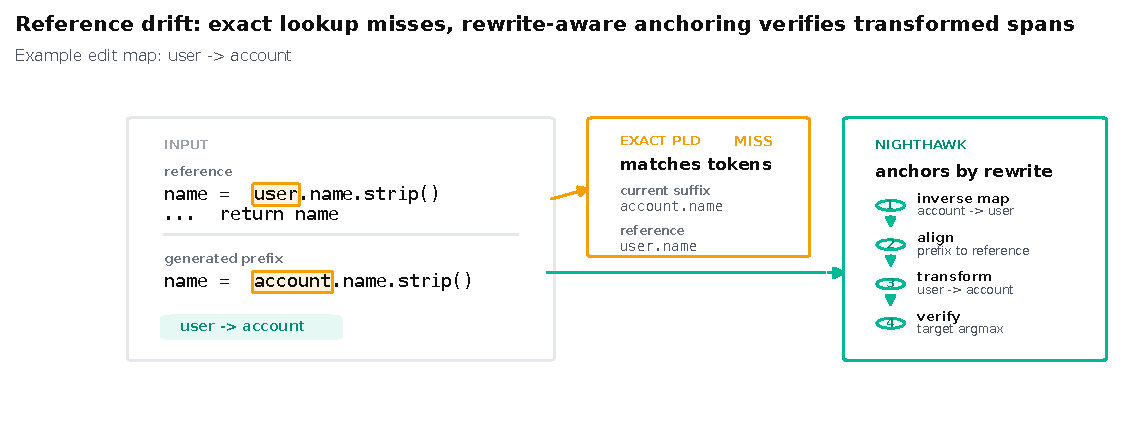
\includegraphics[width=0.95\linewidth]{figures/rewrite_anchor_diagram.pdf}
\caption{Exact PLD copies surface recurrence. Rewrite-View Lookup indexes a
prompt-defined transformed reference, so systematic edits can still
produce exact lookup matches in the target-side view. The deterministic
greedy-equivalence claim is restricted to audited fp32 paths; bf16 timing
is measured separately and is not used for exactness claims.}
\label{fig:rewrite-view}
\end{figure}

\begin{lstlisting}[basicstyle=\ttfamily\scriptsize,frame=single,caption={The validated two-view instance: VANTAGE with SafeRoute, using Rewrite-View Lookup. In the pseudocode, RewriteView denotes the token index built by Rewrite-View Lookup. The view-based algorithm is greedy-equivalent under an exact deterministic target oracle; implementation audits pass on fp32/eager and fp32/sdpa for the controlled rewrite-view workloads. It does not implement sampling-preserving speculative sampling.},label={alg:frozen}]
Input:
  prompt tokens P, reference text R, max_new_tokens L, eos set E
  exact PLD window w=128, exact match n=10

Setup:
  phi = extract_explicit_rewrites(raw_prompt_text)
  if not phi:
      return ExactPLD(P, L, E, w=128, n=10)

  T = apply_boundary_rewrites(R, phi)
  V = tokenize_whole(T)
  if T == R or V == tokenize_whole(R):
      return ExactPLD(P, L, E, w=128, n=10)

  I = build_ngram_index(V, min_match=4, max_match=10)
  prefix = P
  generated = []
  cache = prefill_target_cache(P)

Decode step:
  # Bring the target cache to prefix and get root logits. This is the
  # ordinary target root step shared by exact PLD and VANTAGE/SafeRoute, not a
  # rewrite-view proposal pass.
  root_logits, cache = ensure_target_cache_and_root_logits(prefix, cache)
  g = argmax(root_logits)

  # The proposal is root-excluded. Lookup uses prefix+[g] because g is
  # the target root token and proposed tokens begin after that token.
  exact = ExactPLD.candidate(prefix + [g], w=128, n=10)
  rewrite = RewriteView.candidate(prefix + [g], I, w=128)
  draft = choose_root_excluded_draft(exact, rewrite, tie_break="exact_pld")

  # One verifier call checks [g] + draft. The root g is accepted by
  # construction; logits[j] predicts draft[j] for root-excluded position j.
  verifier_input = [g] + draft
  logits, new_kv = target_forward_with_cache(cache, verifier_input)
  # Under the harness convention, logits has length 1 + len(draft):
  # logits[0] predicts draft[0], and logits[len(draft)] predicts
  # the post-draft bonus token.
  emitted = [g]

  for j in range(len(draft)):
      pred = argmax(logits[j])
      if draft[j] == pred:
          emitted.append(draft[j])
          continue

      # Partial accept. If j == 0, this is token0 reject of the
      # root-excluded draft. The correction was not in verifier_input,
      # so its KV is not kept; it is caught up at the next step.
      correction = pred
      emitted.append(correction)
      keep = 1 + j                 # root plus accepted draft tokens
      cache = crop_to_prefix_plus(cache, new_kv, keep_tokens=keep)
      goto EMIT

  # Full accept. The verifier also gives the next greedy token after the
  # final accepted draft token. This bonus token was not an input token,
  # so its KV is caught up at the next step.
  bonus = argmax(logits[len(draft)])
  emitted.append(bonus)
  keep = 1 + len(draft)            # root plus full draft
  cache = crop_to_prefix_plus(cache, new_kv, keep_tokens=keep)

EMIT:
  emitted = truncate_after_first_eos(emitted, E)
  emitted = truncate_to_remaining_budget(emitted, L - len(generated))
  append emitted to generated and prefix
  if emitted ended with EOS or len(generated) == L: stop
  otherwise continue
\end{lstlisting}

\subsection{Verifier correctness invariant}
\label{sec:correctness}

All methods in the controlled comparison use the same tokenizer, prompt
template, maximum generation cap, EOS/stop policy, sampling parameters
set to deterministic greedy decoding, dtype/backend within a given audit
or timing row, and target-model weights. The only changed object is the
source of proposed root-excluded draft tokens. The proof does not depend on
the draft source being a rewrite view: the same invariant would apply to any
deterministic hidden view implemented with the same verifier contract. In this
paper, implementation evidence is provided only for the identity and rewrite
views used by VANTAGE/SafeRoute.
The standalone PLD comparator in the primary experiments uses the same root
step, cache catch-up, EOS policy, and max-token policy as VANTAGE/SafeRoute;
only the proposal source differs.

\paragraph{Root token and lookup query.}
The notation $g=\arg\max M(\mathrm{prefix})$ denotes the greedy root
token for the current decode step. In the implementation this root
comes from the ordinary target root/catch-up step that maintains the
target cache and computes the next-token logits for the current prefix.
It is therefore not a rewrite-view proposal pass and not a method-specific
extra computation; exact PLD and VANTAGE/SafeRoute both use the same root step.
After $g$ is known, the verifier call consumes \texttt{[g] + draft} in
one batched verifier pass to verify the root-excluded draft and to
produce either a mismatch correction or the full-accept bonus token.
Lookup uses \texttt{prefix + [g]} because the identity/rewrite-view candidate
is root-excluded: it proposes tokens after the verified root token, not
including the root itself. This convention keeps exact PLD and VANTAGE/SafeRoute
on the same verifier interface.

\paragraph{Cache update.}
The target cache is advanced only through target-input tokens whose K/V
entries correspond to the emitted prefix. On full acceptance, the cache
keeps the verifier K/V entries for the root and all draft tokens; the
bonus token is emitted from the final verifier logit but was not an input
token, so its K/V is computed by the next step's catch-up. On partial
acceptance after $a$ accepted root-excluded draft tokens, the cache keeps
the root and the accepted draft prefix; the correction token at the first
mismatch was not an input token, so its K/V is also caught up next step.
On token0 rejection of the root-excluded draft, the cache keeps only the
root and discards all draft K/V entries. EOS is handled after emission by
truncating at the first emitted EOS token, and the global maximum
generation cap truncates the final emitted suffix in the same way for all
methods. Thus the next target forward is always conditioned on exactly the
emitted prefix, even if the previous verifier call evaluated additional
rejected draft tokens.

\paragraph{Greedy-equivalence proof.}
The mathematical statement is an oracle-level statement, not a claim about all
floating-point execution schedules.
The mathematical statement assumes an exact deterministic target next-token
oracle: for a fixed prompt, emitted prefix, tokenizer, model weights, EOS
policy, and max-token cap, verifier logits and argmaxes are invariant to cache
schedule, batch shape, draft length, view choice, and attention kernel. Under
that assumption, prove by induction on decode steps that the decoder's prefix
equals vanilla greedy decoding. The base case holds because both start from
the same prompt tokens. Assume the prefixes are equal at the start of a step.
The verifier computes the same root logits vanilla greedy would compute, so
the emitted root token $g$ is the vanilla greedy next token. The scheduler may
choose any root-excluded draft from any deterministic view. Each accepted draft
token is emitted only after it equals the target greedy argmax at that
position. At the first root-excluded mismatch, including token0 rejection of
the draft, the decoder emits the target argmax correction, which is exactly the
vanilla greedy next token. On full acceptance, the verifier's final logit emits
the next vanilla greedy bonus token. Therefore the emitted block is a prefix of
the vanilla greedy continuation, optionally followed by the next vanilla greedy
correction or bonus token; the updated prefix again equals vanilla greedy. By
induction, the full output is greedy-equivalent until EOS or the shared
max-token cap. View construction and scheduling can only change which draft is
tested, not which verified tokens are emitted.
This paper does not implement or claim preservation of a stochastic
sampling distribution; all correctness claims are deterministic greedy
equivalence claims.

This correctness statement is implementation-audited, not assumed, for the
reported backends. fp32/eager and fp32/sdpa passed byte-identity audits on the
controlled workloads. The bf16 optimized timing runs are not claimed
byte-identical: parity diagnosis found one field task where VANTAGE/SafeRoute diverges
from vanilla/PLD despite taking only exact-PLD/fallback routes, and
identifier-style raw-output divergences tied to max-token continuations.
Backend isolation shows fp32/sdpa passes on the audited rows while bf16/eager
drifts, so the current evidence points to bf16 numerical sensitivity rather
than SDPA alone. These failures are unacceptable for deployment until closed,
so we use bf16/sdpa only for timing diagnostics.

% -----------------------------------------------------------------------------
\section{Experimental Setup}
\label{sec:setup}

\paragraph{Models and hardware.}
The headline exact-path results use \texttt{Qwen/Qwen2.5-Coder-7B} on a single
Modal L40S GPU. The validation logs resolve both model and tokenizer
files to Hugging Face revision
\texttt{0396a76181e127dfc13e5c5ec48a8cee09938b02}. The main throughput
table uses the fp32/sdpa backend-isolation artifact because both PLD and
VANTAGE/SafeRoute match vanilla on 100/100 tasks in every controlled workload.
Correctness audits also include fp32/eager. The bf16 optimized paths have
observed parity drift, so bf16/sdpa is reported only as a timing diagnostic
and is not used to support greedy-equivalence claims.
Sensitivity rows use
\texttt{Qwen/Qwen2.5-Coder-7B-Instruct} and
\texttt{deepseek-ai/deepseek-coder-6.7b-instruct}.

\paragraph{Controlled mechanism benchmark.}
The four headline workloads are controlled Python edit manifests:
zero drift (verbatim/reference target), field substitution, identifier-style substitution, and
a mixed zero/field/identifier-style suite. Each final Qwen-base run uses $n=100$
from four locked files under \path{data/manifests_frozen_audit/}.
The deterministic edited target is stored for analysis but never
included in the prompt or used by SafeRoute. The BlazEdit-style PLD discussion
in Section 2 motivates tuned long-window PLD as the literal-copy comparator
used in the headline rows.
The prompt-router rule and candidate-competition margin were selected
on a disjoint 150-task fitting set; all headline $n=100$ results use
held-out manifests.
Table \ref{tab:controlled-manifest-audit} summarizes the locked manifests.
These are controlled mechanism workloads: field rows use one explicit dotted
field substitution, identifier-style rows use one explicit identifier-style substitution,
and mixed rows combine no-map controls with those two explicit rewrite types.
The deterministic target in each structured row is produced by applying the
rewrite map to the reference. The timing tables run the full locked manifests;
they are not post-hoc filtered by whether the model's raw output exactly
matches the deterministic target. That compliance/task-quality question is
reported separately in Appendix \ref{app:strict-quality}.

\begin{table}[h]
\centering\scriptsize
\caption{Controlled manifest audit generated from the locked validation
manifests. Prompt-visible maps count rows where an explicit non-empty map is
present in the prompt. These rows define the mechanism benchmark, not a
real-commit benchmark.}
\label{tab:controlled-manifest-audit}
\resizebox{\linewidth}{!}{%
\begin{tabular}{lrrrrrrr}
\toprule
Workload & $n$ & Rewrite rows & No-map rows & Target differs & Prompt-visible maps & Pair types & Mean copied \% \\
\midrule
Zero drift & 100 & 0 & 100 & 0 & 0 & none & 100.0 \\
Field substitution & 100 & 100 & 0 & 100 & 100 & dotted field & 98.6 \\
Identifier-style substitution & 100 & 100 & 0 & 100 & 100 & identifier style & 97.3 \\
Mixed & 100 & 66 & 34 & 66 & 66 & 33 field, 33 identifier-style & 98.6 \\
\bottomrule
\end{tabular}}
\end{table}

\paragraph{Metrics.}
We report direct within-run speedup against tuned
\texttt{blazedit\_pld\_w128\_n10}, task-bootstrap 95\% confidence
intervals, tokens per verifier step, verifier-step reduction,
rewrite-view setup diagnostics, SafeRoute route counts, rewrite-view hit
yield, vanilla-output parity, and strict
fp32 byte identity. Strict exact-target/syntax checks are reported only as
appendix diagnostics because the timing artifacts contain raw fenced snippets
and fragmentary completions; they are task-quality diagnostics rather than
decoder-equivalence evidence.

\paragraph{Timing and statistics.}
All methods use the same maximum generation cap of 256 new tokens,
EOS token ID 151643, no chat template, and deterministic greedy
argmax decoding; the paper does not evaluate stochastic sampling.
Tokens/sec is generated tokens divided by decoder wall time. For
VANTAGE/SafeRoute, decoder wall time includes rewrite extraction,
transformed-reference materialization, whole-reference tokenization, index
construction, lookup/routing, verifier computation, cache
crop/catch-up, and hidden-view setup. Prompt tokenization of the original
visible prompt and final text decoding are excluded for all methods, as are
post-hoc stop-string truncation and table/scoring scripts. Target prompt
prefill/cache construction is included in decoder wall time for all methods.
The harness calls \texttt{torch.cuda.synchronize()} before
each task; no separate warmup pass is recorded in the artifact. All
headline comparisons are within-run; confidence intervals are paired
percentile CIs from 5000 task-bootstrap resamples with seed 123, where
each resample draws the same task rows for the compared methods. These CIs
measure task heterogeneity, not run-to-run GPU timing variance; repeated
warmup/randomized-order timing is not measured in the current artifact and is
listed as required future systems validation.

\paragraph{Artifact provenance.}
The validation source of truth is
\path{artifacts/vantage_transpld/validation_manifest.json}. The exact-path
headline and successful-edit slices are regenerated from the backend-isolation
artifact by \path{scripts/summarize_transpld_exact_path_success.py}. The
primary same-policy ablation is regenerated from
\path{artifacts/vantage_transpld/tables/same_policy_fp32_sdpa_20260521_v1/}.
Older bf16 timing tables, controlled-manifest audits, prompt injection
summaries, ViewBank diagnostics, and the deterministic rewrite sanity check are
each regenerated by the scripts and artifact paths listed in
Appendix ``Artifacts and run tags'' and in
\path{docs/vantage_claim_ledger.md}.

\paragraph{Code and artifacts.}
The decoder implementation, locked manifests, paper source, and reproduction
scripts are available at
\url{https://github.com/faizancodes/vantage-rewrite-views}. Large generated
artifacts are intended for a Hugging Face dataset release; until that dataset is
published, the repository documents the exact upload and download plan.

% -----------------------------------------------------------------------------
\section{Primary Controlled Evidence}
\label{sec:results}

\subsection{Rewrite-map views explain controlled structured edit speedups}

Table \ref{tab:frozen-headline} is the main result. On controlled
structured Python edit workloads built around prompt-visible explicit
rewrite maps, SafeRoute routes zero-drift prompts to the
identity PLD view and uses Rewrite-View Lookup only on explicit drift.
The mechanism is best read through three
separate measurements: exact synthetic-target match, local rewrite
compliance, and verifier acceptance of rewrite-view spans. The speedup
claim is driven by the third measurement, not by assuming full edit-task
success; exact-target and syntax diagnostics show that this is not a broad
edit-quality benchmark.
The zero-drift route performs no rewrite-view work and stays near PLD.
We report it as a control row, not as a rewrite-view speedup.

\begin{table}[h]
\centering\scriptsize
\caption{Main exact-path controlled result: VANTAGE with the
SafeRoute scheduler on Qwen2.5-Coder-7B
controlled structured Python edit workloads under fp32/sdpa. Non-control
ratios are paired task-bootstrap comparisons against tuned PLD in the same run; both
PLD and VANTAGE/SafeRoute match vanilla greedy on 100/100 tasks in every row.
For zero drift, the measured ratio is shown only as a same-route measurement
control and its interval is suppressed; because SafeRoute dispatches to the
same PLD path and no rewrite-view index is built, this row is not used as
algorithmic speedup evidence. Bootstrap intervals measure task heterogeneity
within this single run, not run-order or GPU timing variance.}
\label{tab:frozen-headline}
\resizebox{\linewidth}{!}{%
\begin{tabular}{lrrrrrll}
\toprule
Workload & $n$ & PLD tok/s & VANTAGE/SR tok/s &
VANTAGE/SR / PLD & 95\% CI & Parity & Reading \\
\midrule
Zero drift & 100 & 319.9 & 324.7 & 1.015 (control) & -- & 100/100 & same-route PLD control; not a speedup claim \\
Field substitution & 100 & 217.1 & 276.8 & \textbf{1.275} & [1.202,1.358] & 100/100 & explicit field map helps \\
Identifier-style substitution & 100 & 164.9 & 270.3 & \textbf{1.639} & [1.475,1.825] & 100/100 & strongest win \\
Mixed zero/field/identifier-style & 100 & 204.8 & 271.9 & \textbf{1.328} & [1.207,1.482] & 100/100 & mixed-regime win \\
\bottomrule
\end{tabular}}
\end{table}

The faster bf16/sdpa artifacts are now treated only as optimized timing
diagnostics: they report higher absolute token rates but rare raw-output
drift on field and identifier-style rows. This ordering keeps the main
throughput claim on an audited exact path and leaves bf16 deployment as an
open engineering issue.

\subsection{Same-backend same-policy lookup ablation}
\label{sec:same-policy}

A reviewer-visible confound is that the validated Rewrite-View Lookup path uses a
minimum transformed match length of 4 and maximum match length of 10, whereas
the tuned PLD comparator is reported as \texttt{w128,n10}. Table
\ref{tab:same-policy} addresses the main lookup-policy ablation on the same
fp32/sdpa backend and locked $n=100$ manifests. The identity-view
\texttt{m4,n10} row reuses the same min/max lookup policy over the literal
reference; the rewrite-view row changes only the hidden draft source.
Every displayed method matches vanilla greedy on 100/100 prompts in every
workload.

The field and identifier-style rows isolate Rewrite-View Lookup on
effective-map tasks. The mixed row is a mixed-regime suite with both
effective-map rows and no-map controls, so it measures suite-level behavior
rather than a pure rewrite-view effect. The rewrite view beats same-policy
identity lookup by 1.46$\times$ on field substitution and 2.23$\times$ on
identifier-style substitution; the mixed suite shows a 1.66$\times$ suite-level
advantage. The same-policy routed rewrite-view row also beats identity
\texttt{m4,n10} on these rows. This addresses the strongest lookup-policy confound on the
fp32/sdpa backend used for the primary claim: under a matched min/max lookup
policy, the rewrite view substantially outperforms identity-view lookup on
effective-map tasks and remains positive on the mixed suite.
For compact table labels, \textsc{RewriteView} denotes the rewrite-view
candidate source produced by Rewrite-View Lookup, and ``Routed RewriteView''
denotes the same-policy SafeRoute variant.
The zero-drift manifest has no rewrite maps, so same-policy view comparisons
are meaningful only on field, identifier-style, and mixed rows; fallback
behavior on zero drift is covered by the main same-route control.

\begin{table}[h]
\centering\scriptsize
\caption{Same-backend same-policy lookup ablation on structured rows and the
mixed suite under the audited fp32/sdpa path.
Identity PLD and Rewrite-View Lookup use the same
\texttt{min\_match=4,max\_match=10} policy. Ratios are computed from displayed
denominators in the same artifact. CIs are paired task-bootstrap intervals from
5000 resamples with seed 123 and measure task heterogeneity, not run-to-run GPU
variance. The zero-drift fallback row is omitted because no rewrite map exists
there; field and identifier-style rows isolate Rewrite-View Lookup, while mixed
reports suite-level behavior.}
\label{tab:same-policy}
\resizebox{\linewidth}{!}{%
\begin{tabular}{lrrrrrrrl}
\toprule
Workload & Tuned PLD & Identity m4 & Rewrite-view m4 & Routed rewrite-view m4 &
Rewrite-view/identity & Routed/identity & Routed/tuned & Parity \\
\midrule
Field substitution & 222.8 & 185.7 & 270.4 & 243.4 & 1.456 [1.302,1.630] & 1.311 [1.192,1.430] & 1.093 [0.990,1.195] & all 100/100 \\
Identifier-style substitution & 161.7 & 132.9 & 296.4 & 274.6 & 2.230 [1.893,2.630] & 2.066 [1.863,2.287] & 1.698 [1.528,1.881] & all 100/100 \\
Mixed & 205.7 & 167.5 & 277.5 & 261.1 & 1.656 [1.432,1.939] & 1.558 [1.412,1.743] & 1.269 [1.154,1.409] & all 100/100 \\
\bottomrule
\end{tabular}}
\end{table}

The field and identifier-style rewrite-view m4 rows isolate Rewrite-View Lookup
on effective-map tasks. The mixed row includes no-map controls and therefore
reports suite-level behavior. The routed rewrite-view m4 row adds candidate
competition and fallback policy. The routed same-policy
row is not the frozen final decoder: it deliberately matches the identity and
rewrite lookup policies to isolate the view effect. The final VANTAGE/SafeRoute
row keeps the tuned PLD identity branch used in the headline comparator.
Regenerated from the same-policy artifact, the direct
rewrite-view m4 row records 217/185 rewrite-view hits and 14,988/16,056
accepted non-root tokens for field and identifier-style, respectively; the
mixed suite records 134 hits and 10,295 accepted non-root tokens,
confirming that the matched-policy gap corresponds to verifier-accepted
rewrite-view continuations rather than only setup or wrapper effects.

\subsection{Mechanism counters, tail latency, and view-scheduler regressions}

Table \ref{tab:frozen-systems} gives the exact-path mechanism interpretation.
SafeRoute produces the routing safety story on zero drift: every
decode step takes the exact PLD route. On structured edit regimes,
the rewrite-view route is selected on a minority of decode steps but yields
long accepted continuations, cutting the number of verifier steps by
44.7--66.3\%. The verifier-step columns count
logged decode/verification steps under the shared root/catch-up convention, not
raw GPU kernel launches; PLD and VANTAGE/SafeRoute use the same root step, cache
catch-up, EOS policy, and max-token policy. This is the central
evidence that the speedup comes from turning prompt-visible rewrites into
copyable spans; Section \ref{sec:same-policy} separates this mechanism
from match-policy effects.
Accepted per rewrite-view hit is high because the explicit rewrite materializes
the target-side reference view: once a suffix match lands in that view,
the following rewrite-view span often remains aligned for tens of tokens.
The value is still bounded by the \texttt{w128} draft window, remaining
generation budget, EOS/max-token handling, and the verifier's first
target-argmax rejection. We do not interpret these long-hit statistics
as evidence for broad real-commit generalization; they characterize the
controlled structured synthetic regimes in this validation.

A simple cost model summarizes when the mechanism should help. Let
$S_{\text{view}}$ be one-time rewrite, whole-reference tokenization, and
index-construction cost, $\Delta C_{\text{lookup}}$ the extra lookup/routing
cost over PLD, and $C_{\text{verify}}$ the average cost of one target
verification step. VANTAGE/SafeRoute should improve over PLD on a task when its rewrite-view
savings satisfy
\[
(N_{\text{steps,PLD}}-N_{\text{steps,SR}})C_{\text{verify}}
>
S_{\text{view}}+\Delta C_{\text{lookup}}.
\]
The tail regressions in Table \ref{tab:tail-regression} are the task-level
cases where this inequality fails despite holding in aggregate.
This explains why the method depends on long verifier-accepted rewrite-view
spans, why zero-drift prompts should route back to PLD, and why short or
low-acceptance rewrite-view proposals create tail regressions.

\begin{table}[h]
\centering\scriptsize
\caption{Mechanism counters from the Qwen-base fp32/sdpa exact-path
$n=100$ validation. Verifier steps count logged decode/verification steps
under the shared root/catch-up convention, not raw GPU kernel launches.
RewriteView hits count selected rewrite-view proposals; accepted/hit
counts accepted non-root tokens from those hits. In route counts, ``no draft''
denotes decode steps with no selected non-root draft beyond the verified root.}
\label{tab:frozen-systems}
\resizebox{\linewidth}{!}{%
\begin{tabular}{lrrrrrrrl}
\toprule
Workload & Gen. tok. & PLD verifier steps & VANTAGE/SR verifier steps &
Step red. & RewriteView hits & RewriteView acc. & Accepted/hit & Route counts \\
\midrule
Zero drift & 14769 & 506 & 506 & 0.0\% & 0 & 0 & 0.00 & PLD 506 \\
Field substitution & 15524 & 752 & 388 & 48.4\% & 63 & 6422 & 101.94 & PLD 256, RewriteView 63, no draft 69 \\
Identifier-style substitution & 16660 & 1200 & 404 & 66.3\% & 104 & 9413 & 90.51 & PLD 268, RewriteView 104, no draft 32 \\
Mixed & 16224 & 901 & 498 & 44.7\% & 61 & 5772 & 94.62 & PLD 408, RewriteView 61, no draft 29 \\
\bottomrule
\end{tabular}
}
\end{table}

Equivalently, structured rows raise generated tokens per verifier step from
20.6 to 40.0 on field substitution, 13.9 to 41.2 on identifier-style
substitution, and 18.0 to 32.6 on mixed.
The exact-path tail table shows that SafeRoute is an aggregate guard, not a
per-task dominance theorem. The fp32/sdpa control row has 9/100 regressions
and a worst task ratio of 0.983$\times$, consistent with
near-parity same-route behavior rather than a rewrite-view speedup.
Structured rows still have tail risk: identifier-style substitution has a
strong median win (1.746$\times$) but a worst observed exact-path slowdown of
0.716$\times$, and mixed has a similar worst slowdown. These regressions are
material for interactive use and motivate better adaptive routing.

\paragraph{Tail latency and regressions.}
SafeRoute improves aggregate throughput on structured workloads, but it is
not a per-task dominance guarantee. The generated regression table in
\path{artifacts/vantage_transpld/tables/exact_path_success_20260518_v1/}
reports per-task speedup percentiles, p50/p95/p99 VANTAGE/SafeRoute latency, worst
slowdown, and whether a regressing task used a rewrite-view route. Table
\ref{tab:tail-regression} summarizes the fp32/sdpa exact-path tail diagnostics.
We keep these diagnostics in the main text because interactive code-edit
systems care about regressions even when aggregate throughput improves.

\begin{table}[h]
\centering\scriptsize
\caption{Per-task tail and regression diagnostics against tuned PLD on the
same fp32/sdpa exact path as Table \ref{tab:frozen-headline}. Speedup ratios
are computed per task from generated-token tok/s. RewriteView-route regressions
count tasks with at least one rewrite-view route and per-task speedup below
1.}
\label{tab:tail-regression}
\resizebox{\linewidth}{!}{%
\begin{tabular}{lrrrrl}
\toprule
Workload & Regressions & RewriteView-route regressions & VANTAGE/SR p99 ms &
Worst task ratio & Per-task speedup p05/p50/p95 \\
\midrule
Zero drift & 9/100 & 0/0 & 2600.8 & 0.983$\times$ & 0.996/1.020/1.044 \\
Field substitution & 13/100 & 6/50 & 1741.8 & 0.868$\times$ & 0.956/1.270/2.621 \\
Identifier-style substitution & 17/100 & 12/85 & 1630.0 & 0.716$\times$ & 0.809/1.746/3.201 \\
Mixed & 9/100 & 5/49 & 2832.7 & 0.715$\times$ & 0.989/1.162/2.849 \\
\bottomrule
\end{tabular}}
\end{table}


\subsection{Backend parity audit and edit quality}

The verifier-correctness claim is separate from edit-task quality.
Table \ref{tab:quality} separates audited fp32 byte identity from bf16/sdpa
timing-path parity, and Table \ref{tab:backend-audit} summarizes the broader
backend matrix. The greedy-equivalence claim is restricted to audited fp32
paths: PLD and VANTAGE/SafeRoute match vanilla greedy on every audited controlled
workload under both fp32/eager and fp32/sdpa. The bf16/sdpa rows are optimized
timing runs and show rare raw-output drift. The known field mismatch occurs on
an exact-PLD/fallback-routed task, not after a rewrite-view route; the identifier-style
raw mismatches are max-token continuations.

We treat the controlled validation suite as a \emph{mechanism benchmark}: it
tests whether rewrite views create accepted copy spans and whether the
decoder preserves the target verifier's greedy output. It is not yet a strong
edit-quality benchmark. Appendix \ref{app:strict-quality} diagnoses the
separate exact-target and Python-syntax checks. In particular, the earlier
identifier-style 0.0\% syntax report came from scoring stored Markdown-fenced
snippets without extracting the code block; after extracting code from
\texttt{raw\_text}, identifier-style substitution reaches 68.0\% exact target and 79.0\%
syntax for all three decoders, with remaining failures dominated by incomplete
256-token continuations and strict target mismatches.

\begin{table}[h]
\centering\scriptsize
\caption{Decoder parity on headline workloads. Greedy equivalence is claimed
for the audited fp32/eager and fp32/sdpa columns. The bf16/sdpa columns are
timing-path diagnostics and contain observed rare raw-output drift. Strict
target/syntax checks are appendix diagnostics.}
\label{tab:quality}
\resizebox{\linewidth}{!}{%
\begin{tabular}{lrrrrrr}
\toprule
Workload & PLD=vanilla bf16/sdpa & VANTAGE/SR=vanilla bf16/sdpa & PLD fp32/eager & VANTAGE/SR fp32/eager & PLD fp32/sdpa & VANTAGE/SR fp32/sdpa \\
\midrule
Zero drift & 100.0\% & 100.0\% & 100/100 & 100/100 & 100/100 & 100/100 \\
Field substitution & 100.0\% & 99.0\% & 100/100 & 100/100 & 100/100 & 100/100 \\
Identifier-style substitution & 98.0\% & 99.0\% & 100/100 & 100/100 & 100/100 & 100/100 \\
Mixed & 100.0\% & 100.0\% & 100/100 & 100/100 & 100/100 & 100/100 \\
\bottomrule
\end{tabular}}
\end{table}

\begin{table}[h]
\centering\scriptsize
\caption{Backend audit status. The theorem and implementation audit cover the
deterministic fp32/eager path. fp32/sdpa also passed this isolation audit. bf16
paths remain parity-drifting, so bf16/sdpa throughput rows are timing
diagnostics rather than exactness evidence.}
\label{tab:backend-audit}
\setlength{\tabcolsep}{3pt}
\begin{tabular}{@{}L{0.13\linewidth}L{0.14\linewidth}L{0.43\linewidth}L{0.25\linewidth}@{}}
\toprule
Execution path & Purpose & Current evidence & Paper claim \\
\midrule
fp32/eager & theorem audit & PLD and VANTAGE/SafeRoute 100/100 on zero/field/identifier-style/mixed & greedy-equivalence evidence \\
fp32/sdpa & attention isolation & PLD and VANTAGE/SafeRoute 100/100 on zero/field/identifier-style/mixed & measured exactness only for this audit \\
bf16/sdpa & timing path & zero/mixed 100/100; field and identifier-style VANTAGE/SafeRoute 99/100 & speed diagnostic, not exactness evidence \\
bf16/eager & dtype isolation & drift on every workload; VANTAGE/SafeRoute ranges 91--98/100 & bf16 numerical sensitivity evidence \\
\bottomrule
\end{tabular}
\end{table}


% -----------------------------------------------------------------------------
\section{Diagnostics and Boundaries}
\label{sec:diagnostics}

Appendix Table \ref{tab:successful-slices} shows that the speedup persists
on exact-target, syntax-valid, and rewrite-compliant diagnostic slices.
These post-hoc slices are not used as primary evidence.

\subsection{Preliminary multi-view real-commit timing diagnostic}
\label{sec:mv-real-commit}

In a preliminary bf16/sdpa real-commit diagnostic, the rewrite-view-only variant was
slower than tuned PLD, while several multi-view variants showed
1.02--1.04$\times$ single-run diagnostic speedups with raw-output agreement
against tuned PLD of 976--982/1000. Because this artifact is bf16, drifting,
and single-run, we
treat it only as motivation for exact-path ViewBank validation rather than as
an exact real-commit acceleration claim. Appendix Table
\ref{tab:viewbank-real-commit} reports the full table, including the negative
rewrite-only row.

\paragraph{Prompt-only route-margin ablation.}
Appendix Table \ref{tab:route-margin} reports bf16 route-margin diagnostics.
Stricter prompt-only margins reduce some rewrite-view-route regressions but do
not dominate the frozen margin-0 policy; field and mixed lose aggregate
speedup as the margin rises, while identifier-style keeps its best aggregate
result under margin 0. Because the table is bf16 and parity-drifting, it is not
primary evidence.

\subsection{Prompt injection as a changed-prompt alternative}
A natural reviewer baseline is to put the transformed reference directly
into the prompt and then run PLD under the modified prompt. This is cheap and powerful, but
it changes the visible prompt and therefore the target greedy function.
We implemented this changed-prompt baseline as an $n=100$ bf16/sdpa validation on
zero, field, identifier-style, and mixed manifests. With the transformed reference
visibly inserted, PLD under the modified prompt reaches 950.7 tok/s on field, 1257.3 tok/s
on identifier-style, and 838.2 tok/s on mixed (22.94$\times$, 30.12$\times$, and
20.36$\times$ over vanilla under the modified prompt, with 100/100
PLD--vanilla parity under the modified prompt in each row). The zero-control manifest injects no
additional transformed-reference text and reaches 945.3 tok/s under ordinary PLD. The raw
artifacts and generated summary are in
\path{artifacts/vantage_transpld/tables/prompt_injection_20260516_v1/}.
We report this as a serious changed-prompt practical baseline: the headline
VANTAGE/SafeRoute comparison keeps the original visible prompt fixed and uses derived
views only as internal draft sources. For applications that
permit prompt rewriting and accept changed target outputs, this visible
injection baseline may be the more practical choice on these controlled rows;
VANTAGE targets the stricter fixed-prompt setting. Thus this baseline answers a
different question: how fast generation can be when the task itself is rewritten
into an easier prompt.

\begin{table}[h]
\centering\scriptsize
\caption{Changed-prompt visible transformed-reference baseline, measured on
the bf16/sdpa timing backend. It is faster in absolute tok/s on these
controlled rows, but it changes the prompt and target greedy function; raw
tok/s should not be read as backend-normalized against the fp32/sdpa headline.
Exact target and syntax are computed after raw code-block extraction; rewrite
compliance is a conservative local boundary-aware check from the generated
summary.}
\label{tab:prompt-injection-quality}
\resizebox{\linewidth}{!}{%
\begin{tabular}{lrrrrrr}
\toprule
Workload & Injection PLD tok/s & Speedup vs vanilla (mod. prompt) & Exact target &
Syntax & Rewrite compliance & Output differs from original vanilla \\
\midrule
Zero drift & 945.3 & 21.30 & 77/100 & 83/100 & n/a & 0/100 \\
Field substitution & 950.7 & 22.94 & 80/100 & 83/100 & 100/100 & 24/100 \\
Identifier-style substitution & 1257.3 & 30.12 & 73/100 & 73/100 & 93/100 & 9/100 \\
Mixed & 838.2 & 20.36 & 74/100 & 78/100 & 65/66 & 9/100 \\
\bottomrule
\end{tabular}}
\end{table}

The final column compares the changed-prompt output with vanilla greedy under
the original prompt, illustrating that visible injection changes the target
function even when PLD matches vanilla greedy under the modified prompt.

\subsection{Deterministic rewrite-engine sanity check}

For explicit lexical maps, a deterministic rewrite engine is a natural
task-solver baseline. Table \ref{tab:deterministic-rewrite} applies the same
conservative boundary-aware rewrite function used to construct the Rewrite-View
Lookup hidden view directly to each controlled manifest reference. This is not a
decoder baseline and is not compared by tok/s against PLD or VANTAGE. This baseline
solves the synthetic target, but it does not answer the decoder question studied
here: how to accelerate the target model's original prompt-conditioned greedy
output without changing that prompt. It
exists to make the contribution boundary explicit: VANTAGE accelerates the
target model's fixed-prompt greedy output; it does not claim that applying an
explicit lexical rewrite map requires an LLM.

\begin{table}[h]
\centering\scriptsize
\caption{Deterministic rewrite-engine sanity baseline on the locked controlled
manifests. This is a task-solver sanity check, not a speculative-decoding
baseline. The generated artifact includes descriptive local CPU timings, but
the main table omits them because sub-microsecond no-op timings are below a
meaningful systems-measurement scale. Generated by
\texttt{scripts/summarize\_deterministic\_rewrite\_baseline.py}.}
\label{tab:deterministic-rewrite}
\resizebox{\linewidth}{!}{%
\begin{tabular}{lrrrrr}
\toprule
Workload & Tasks & Rewrite rows & Exact target & Syntax & Rewrite compliance \\
\midrule
Zero drift & 100 & 0 & 100/100 & 100/100 & n/a \\
Field substitution & 100 & 100 & 100/100 & 100/100 & 100/100 \\
Identifier-style substitution & 100 & 100 & 100/100 & 100/100 & 100/100 \\
Mixed & 100 & 66 & 100/100 & 100/100 & 66/66 \\
\bottomrule
\end{tabular}}
\end{table}

This table also makes the controlled benchmark limitation explicit: the
deterministic targets are recoverable by deterministic rewriting, so exact
target-task success is not the claimed contribution.

\subsection{Instruction-compliance boundary}
\label{sec:boundary}

VANTAGE accelerates the target model's realized output; it cannot make
a model follow an edit instruction. We measure compliance as
$d(y,R)/(d(y,R)+d(y,T))$, where $y$ is the model output, $R$ is the
original reference, $T$ is the deterministic rewritten target, and $d$
is token edit distance over lightweight code tokens; larger values mean
the output is closer to the rewritten target. This metric is not a full
edit-quality score; it is a coarse diagnostic for whether the model output
moved toward the rewritten target rather than copying the original reference.
Table \ref{tab:boundary}
shows the resulting boundary. Qwen base is the headline model. Qwen
Instruct preserves the identifier-style win and near-zero behavior but field substitution
is not a clear win. DeepSeek Instruct remains PLD-favored on field/identifier-style.
We therefore do not claim that the speedup transfers across target
models. The per-task compliance correlation is weak or not estimable in
several rows because many identifier-style/zero tasks tie under this metric, so the
scientific boundary is the aggregate model/workload behavior plus the
concrete verifier rejections below, not a universal monotone law.
The instruct-model rows use the same raw edit prompt format and no chat
template for comparability with the base-model controlled manifests; they are
therefore sensitivity diagnostics, not a fair deployment evaluation of
instruction-tuned chat prompting.

A representative DeepSeek-Instruct field-rename prompt asks for
\texttt{.renderers} to become \texttt{.renderers\_updated}. Rewrite-View Lookup
proposes the transformed suffix, but the target verifier rejects it
because DeepSeek's greedy output keeps the old field:

\begin{lstlisting}[basicstyle=\ttfamily\tiny,frame=single]
# requested edit
self.renderers  ->  self.renderers_updated

# RewriteView draft at the rewrite frontier
self.renderers_updated

# DeepSeek-Instruct greedy continuation
self.renderers
\end{lstlisting}

In this case, exact PLD is faster because it copies the model's
non-compliant surface form. The same mechanism is why rewrite-view
lookup is best framed as a speedup for models that actually adopt the
prompt-defined rewrite.

\begin{table}[h]
\centering\scriptsize
\caption{Instruction-compliance boundary. Ratios are against tuned PLD.
Qwen-base rows use the audited fp32/sdpa exact-path artifact; instruct rows use
existing untemplated bf16/sdpa boundary artifacts. Spearman correlation is per-task
rewrite-compliance vs. VANTAGE/PLD and is marked n/a when compliance is tied
or missing. Zero-drift rows are same-route controls and are not interpreted as
rewrite-view speedups.}
\label{tab:boundary}
\resizebox{\linewidth}{!}{%
\begin{tabular}{llrrrl}
\toprule
Target & Workload & $n$ & VANTAGE/PLD [95\% CI] & Spearman & Reading \\
\midrule
Qwen2.5-Coder-7B & Field & 100 & 1.275 [1.202,1.358] & 0.317 & structured win \\
Qwen2.5-Coder-7B & Identifier-style & 100 & 1.639 [1.475,1.825] & n/a & compliance tied; structured win \\
Qwen2.5-Coder-7B & Zero & 100 & 1.015 (control) & n/a & PLD-route control; not a speedup claim \\
\midrule
Qwen2.5-Coder-7B-Instruct & Field & 50 & 1.034 [0.940,1.151] & 0.214 & no clear win \\
Qwen2.5-Coder-7B-Instruct & Identifier-style & 50 & 1.437 [1.218,1.712] & n/a & identifier-style survives \\
Qwen2.5-Coder-7B-Instruct & Zero & 50 & 1.003 control [0.998,1.010] & n/a & no rewrite; near PLD \\
\midrule
DeepSeek-Coder-6.7B-Instruct & Field & 50 & 0.879 [0.833,0.916] & 0.038 & PLD favored \\
DeepSeek-Coder-6.7B-Instruct & Identifier-style & 50 & 0.954 [0.901,1.009] & 0.390 & inconclusive/PLD favored \\
DeepSeek-Coder-6.7B-Instruct & Zero & 50 & 1.000 control [1.000,1.000] & n/a & exact route tied \\
\bottomrule
\end{tabular}
}
\end{table}

\begin{figure}[t]
\centering
\begin{minipage}{0.48\linewidth}
\centering
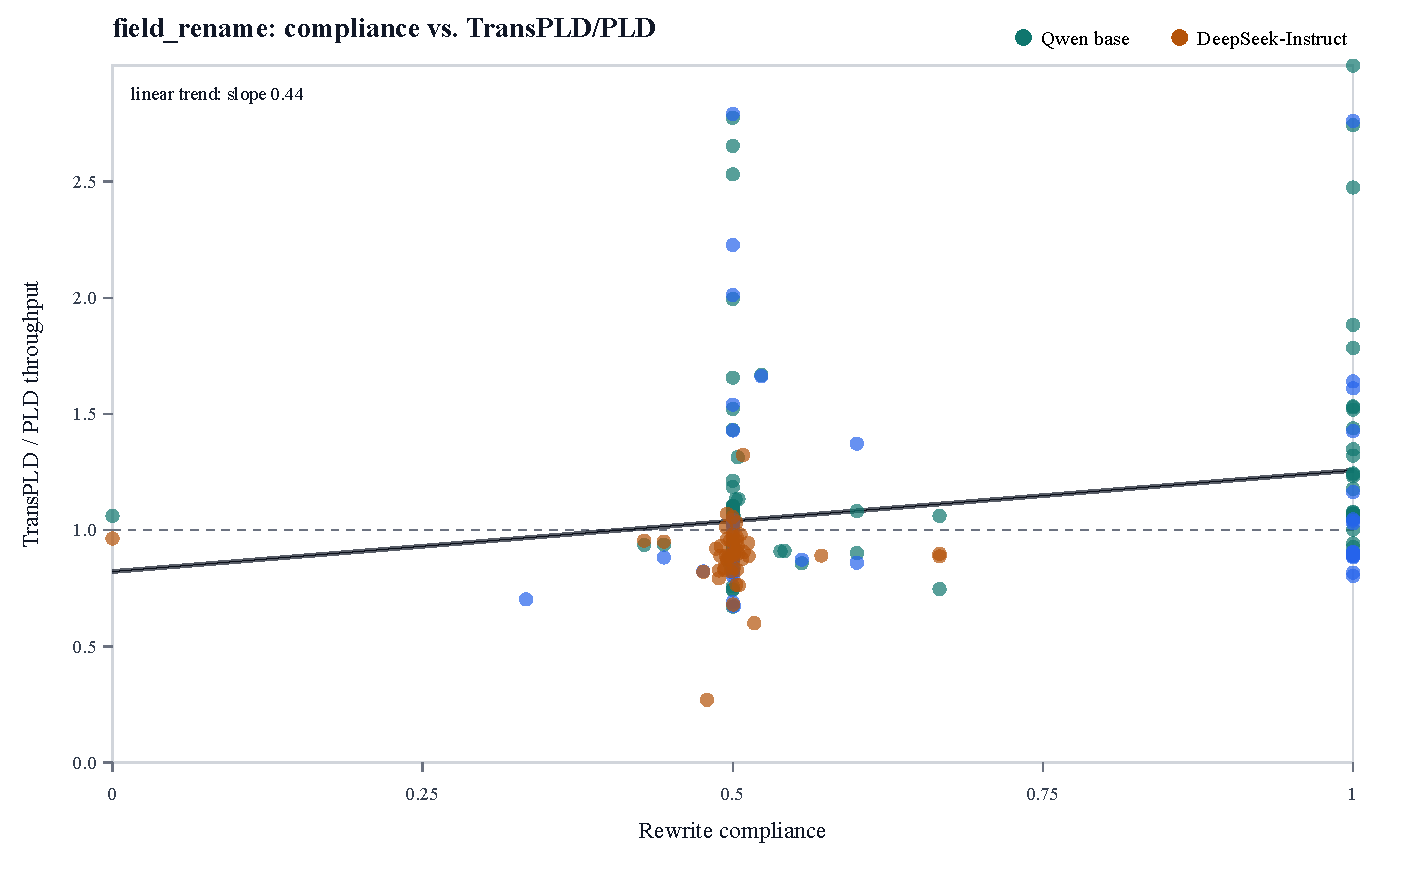
\includegraphics[width=\linewidth]{figures/compliance_field_rename.pdf}
\end{minipage}\hfill
\begin{minipage}{0.48\linewidth}
\centering
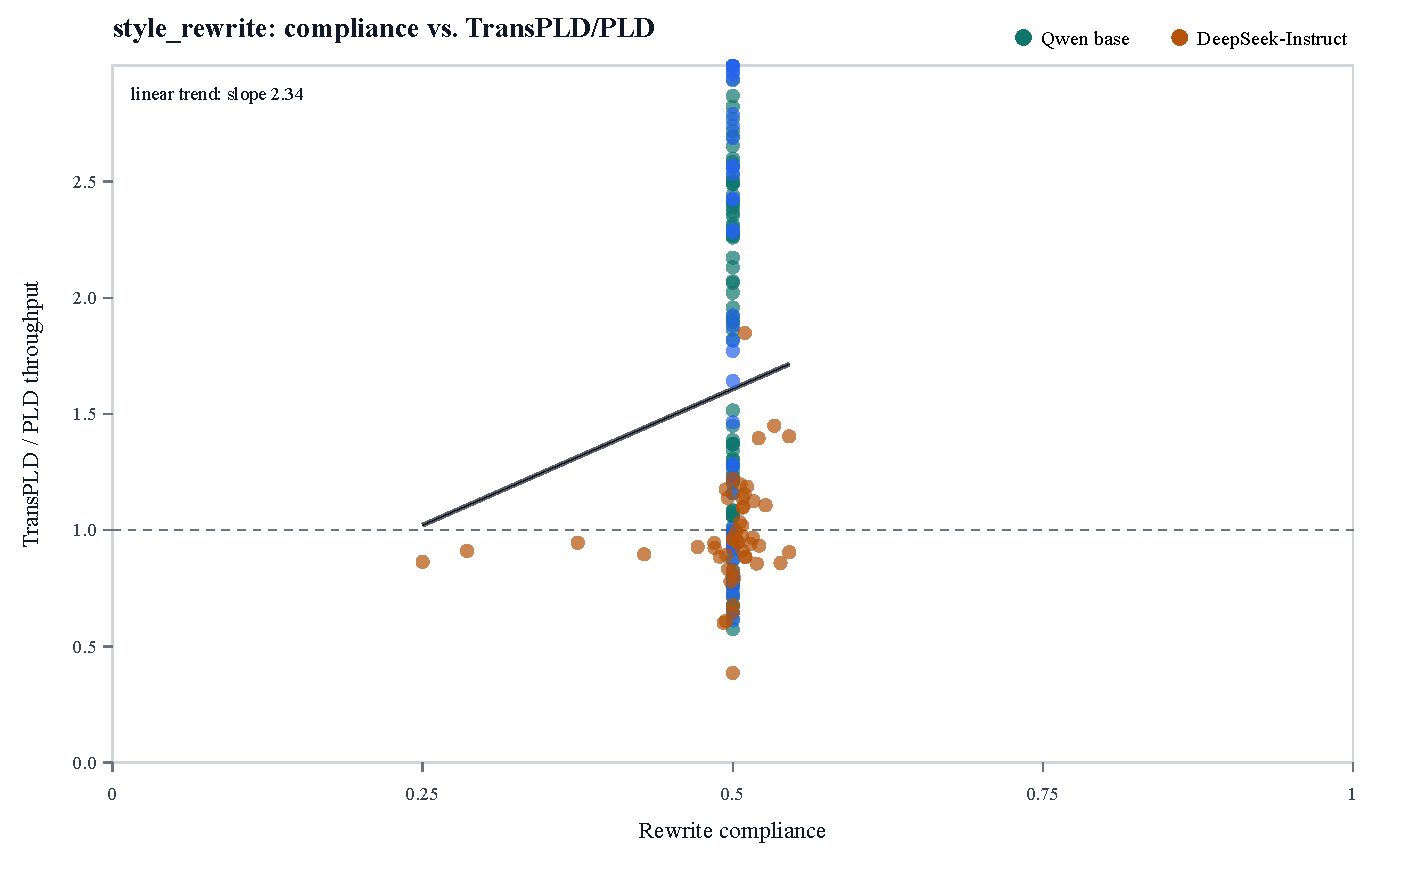
\includegraphics[width=\linewidth]{figures/compliance_style_rewrite.pdf}
\end{minipage}
\caption{Per-task rewrite compliance vs. VANTAGE/PLD ratio in the compliance
boundary artifacts. Higher compliance means the output is closer to the
deterministic rewritten target than to the original reference. The dashed
horizontal line marks parity. The trend is a diagnostic, not a universal law:
field rows show weak positive association for Qwen, while identifier-style/zero rows can
tie under the compliance metric and are marked not estimable.}
\label{fig:compliance}
\end{figure}

% -----------------------------------------------------------------------------
\section{Related Work}

\paragraph{Speculative decoding.}
Classical speculative decoding verifies tokens from a cheaper draft
model against a target model while preserving the target distribution
\cite{leviathan2023,chen2023}. Medusa, EAGLE, EAGLE-2, and Sequoia improve
neural/tree draft mechanisms \cite{cai2024,eagle1,eagle2,chen2024sequoia}.
VANTAGE is orthogonal: it is a model-free hidden-view draft source rather
than a neural draft model. The broader ViewBank scheduler is preliminary
in this paper.

\paragraph{Prompt lookup, n-gram, suffix, and automaton decoding.}
Prompt lookup decoding, vLLM/TensorRT-LLM n-gram speculation,
SuffixDecoding, and SAM-Decoding establish exact context/history reuse as a
strong baseline
\cite{promptlookup,hfpld,vllmngram,tensorrtngram,suffixdecoding,samdecoding}. We
use tuned PLD as the comparator and treat exact lookup as prior art.
Rewrite-View Lookup asks what happens when recurrence appears in a deterministic hidden
rewrite view derived from the prompt rather than in the literal prompt itself.
This places Rewrite-View Lookup between identity-only n-gram reuse and learned
draft models: it remains model-free, but its draft source is not limited to
literal prompt recurrence.
Unlike modifying the model's prompt with rewritten code, VANTAGE constructs an
internal verified draft view; the visible prompt and target greedy function are
unchanged on audited exact paths.
The broader ViewBank framing suggests a code-edit speculative decoding
framework built around deterministic hidden prompt-derived code views with
fixed-prompt target verification. In this paper, only the Rewrite-View Lookup instance
is exact-path validated; the multi-view claim remains diagnostic rather than a
validated systems result.

\paragraph{Code-edit acceleration and BlazEdit.}
BlazEdit targets whole-file code editing with prompt lookup and assisted
decoding, reporting strong acceleration on copy-heavy edit scenarios
\cite{blazedit}. Our comparison is in-harness rather than a reproduction
of the public production stack, but it is consistent with the central lesson:
long-window PLD is the right exact-copy baseline. VANTAGE extends that
baseline by treating PLD as identity-view lookup and adding a hidden rewrite
view when literal recurrence is weak.

\paragraph{EfficientEdit and edit-oriented speculation.}
EfficientEdit is the closest recent work in application scope: it targets
code editing by reusing original code segments, drafting edit content with
edit-oriented draft models, and using dynamic verification to balance
quality and acceleration \cite{efficientedit}. VANTAGE differs in the draft
source and intervention point. It does not train or invoke an edit draft model;
it builds deterministic hidden code views from the prompt and verifies their
drafts with the target model. EfficientEdit is not experimentally compared in this paper.
Accordingly, our measured claim is against tuned PLD in the same research
harness, not against EfficientEdit or production serving stacks.

\begin{table}[h]
\centering\scriptsize
\caption{Baseline positioning. Tuned PLD, VANTAGE/Rewrite-View Lookup, and
preliminary ViewBank variants are measured in our research harness. Visible prompt
injection is a changed-prompt baseline measured separately on $n=100$
manifests; other rows provide related-work context and are not implied
experimental wins.}
\label{tab:baseline-positioning}
\resizebox{\linewidth}{!}{%
\begin{tabular}{llll}
\toprule
Method family & Draft source & Edit-specific mechanism & Role in this paper \\
\midrule
Exact PLD & Original prompt/history n-grams & Literal recurrence only & Main measured comparator \\
Visible transformed-reference prompt injection & Modified prompt contains rewritten reference & Makes the transformed target visibly copyable & Measured $n=100$ changed-prompt baseline; changes target prompt \\
vLLM/TensorRT n-gram & Production n-gram or prompt lookup pools & Exact reuse in serving stacks & Context; not experimentally compared \\
BlazEdit-style PLD & Long-window PLD plus assisted decoding stack & Whole-file edit copy acceleration & Motivation; public stack not reproduced \\
EfficientEdit & Code reuse plus edit-oriented draft models & Reuse-or-generate policy with dynamic verification & Closest edit-specific related work; not experimentally compared \\
VANTAGE / Rewrite-View Lookup & Internal transformed reference view & Rewrite maps turn structured drift into copyable spans & Validated rewrite-view instance \\
Preliminary ViewBank & Deterministic hidden prompt-derived code views & Identity, rewrite, patch/frontier, rescue, cursor, and hunk views & Preliminary framework diagnostics \\
\bottomrule
\end{tabular}}
\end{table}

\paragraph{Serving systems.}
vLLM/PagedAttention and SGLang optimize serving memory, scheduling, and
structured execution \cite{kwon2023vllm,zheng2024sglang}. Our measurements are
from a research harness; integrating rewrite-view lookup into a production
serving stack is future work.

% -----------------------------------------------------------------------------
\section{Discussion and Limitations}
\label{sec:limitations}

\begin{itemize}
\item \textbf{Controlled drift and diagnostic real-commit evidence.} The
  exact-path headline workloads are controlled structured Python drift suites.
  Their deterministic targets are exactly recoverable by the explicit rewrite
  maps, so VANTAGE is not claimed as a better task solver for those lexical
  rewrites.
  The balanced 1000-task multi-view real-commit artifact is a bf16 timing
  diagnostic, not an exact-path deployment result, and its output drift is
  reported in Table \ref{tab:viewbank-real-commit}. The older 33-row
  real-commit pilot in Appendix \ref{app:real-commit-pilot} is inconclusive
  and remains only as provenance for the benchmark protocol. A larger
  preregistered commit benchmark with exact-path validation remains necessary
  before any broad real-commit-quality claim.
\item \textbf{Single headline model and compliance boundary.} The
  positive throughput claim is on Qwen2.5-Coder-7B controlled
  structured Python edit workloads with prompt-visible explicit rewrite
  maps. The mechanism evidence shows that the verifier often accepts long
  rewrite-view spans on those workloads. Instruct-model retests show rewrite-view
  lookup helps only when the target model adopts the rewrite. They did not use
  each model's recommended chat template, so they are sensitivity diagnostics
  rather than a proper instruction-model deployment evaluation. We do not claim
  multi-model universality.
\item \textbf{Not a production-serving or sampling claim.} These
  experiments use a research harness, not a vLLM production-serving
  stack. The verifier audit establishes deterministic greedy-output
  equality under audited fp32 execution; it does not establish
  sampling-distribution preservation.
\item \textbf{bf16 optimized-path parity gap.} The optimized bf16 timing
  paths are not greedy-equivalent in the current artifact. The parity diagnosis
  found rare bf16/sdpa raw-output drift: one field task diverged without using
  a rewrite-view route, and identifier-style raw-output mismatches occurred on
  max-token continuations. The backend-isolation matrix also shows broader
  bf16/eager drift while fp32/sdpa passes, so the evidence points to bf16
  numerical sensitivity rather than SDPA alone. This is not acceptable for
  deployment until the timing path is made byte-identical or the serving stack
  supplies an equivalent deterministic verifier.
\item \textbf{Task quality remains shallow.} We report vanilla-parity,
  exact-target, syntax, and fp32 byte-identity checks, but these are
  diagnostics, not a full edit-quality evaluation. The identifier-style 0.0\%
  syntax row in the earlier strict table was a code-extraction artifact; after
  extracting fenced code from \texttt{raw\_text}, identifier-style syntax is 79.0\% and
  exact target is 68.0\% for all methods. The remaining failures include
  max-token truncation and exact-target mismatches, and real-commit
  exact-target and syntax rates are low. Full benchmark-specific edit success
  or unit-test pass@1 is not integrated.
\item \textbf{Single-run timing.} The current timing artifacts synchronize
  CUDA around each task and use paired task bootstraps, but they do not
  include repeated warmup runs or randomized method order. The confidence
  intervals in the paper quantify task heterogeneity within a run, not
  run-to-run GPU variance.
\item \textbf{Prompt-derived views are conservative.} The rewrite view uses
  conservative explicit rename/replace extraction; implicit semantic
  rewrite-map inference is out of scope. Patch/frontier, rescue, cursor, and
  hunk views are deterministic heuristics in a research harness, not a learned
  production scheduler. Unit tests cover supported view/parser behavior, but
  real-prompt extraction precision/recall remains future work.
\item \textbf{Zero-drift near-parity is not a speedup.} SafeRoute
  performs no rewrite-view work on zero-drift prompts. We report it as
  a control row and do not claim rewrite-view acceleration there. The current
  locked zero-drift control contains no prompt-visible rewrite maps, so it
  validates no-map routing rather than an explicit no-op-map timing control.
\item \textbf{Research-harness timing.} We compare within one verifier
  harness on one GPU. Production batching, public BlazEdit serving-stack
  behavior, vLLM integration, and long-context deployment remain future
  work.
\end{itemize}

% -----------------------------------------------------------------------------
\section{Conclusion}

This paper validates a narrow fixed-prompt mechanism: hidden rewrite views can
restore copyable spans that literal PLD misses, while target verification
preserves deterministic greedy output on audited fp32 paths. VANTAGE is the
validated decoder, and Rewrite-View Lookup is its core primitive. VANTAGE
materializes prompt-visible explicit rewrite maps as a whole-tokenized hidden
reference, uses that reference only as a draft source, and routes no-map
controls back to exact PLD through SafeRoute. On Qwen2.5-Coder-7B controlled
explicit-map Python edit workloads, the audited
fp32/sdpa path is 1.28$\times$ faster than tuned PLD on field substitutions,
1.64$\times$ faster on identifier-style substitutions, and 1.33$\times$ faster
on a mixed structured suite; zero drift is reported only as a same-route PLD
control. The mechanism evidence is direct: structured rows cut verifier steps
by 44.7--66.3\%, and selected rewrite-view proposals accept 91--102 tokens
per hit.

The controlled target itself is deterministic-rewrite recoverable, and that is
not the paper's claimed contribution. The contribution is fixed-prompt
model-output acceleration: when the model would already follow the transformed
reference under the original prompt, the hidden view exposes verified spans
missed by literal PLD.

The broader ViewBank prototype remains preliminary. The balanced real-commit
multi-view artifact is a bf16 single-run timing diagnostic with raw-output
drift, so it is not a primary exact-path or production result; rewrite-view-only
transfer is negative/inconclusive outside the controlled explicit-map
setting. The paper therefore does not claim production serving, sampling
preservation, broad edit-quality improvement, broad real-commit transfer, or
multi-model universality. The immediate next step is to validate richer
prompt-derived views on exact repeated-timing real-edit benchmarks; the present
result establishes the fixed-prompt rewrite-view mechanism in the controlled
regime where literal PLD loses recurrence.

% -----------------------------------------------------------------------------
\bibliographystyle{plain}
\begin{thebibliography}{99}

\bibitem{leviathan2023}
Y.~Leviathan, M.~Kalman, Y.~Matias.
\newblock Fast Inference from Transformers via Speculative Decoding.
\newblock \emph{ICML 2023}.

\bibitem{chen2023}
C.~Chen, S.~Borgeaud, G.~Irving, J.-B.~Lespiau, L.~Sifre, J.~Jumper.
\newblock Accelerating Large Language Model Decoding with Speculative Sampling.
\newblock \emph{arXiv:2302.01318}, 2023.

\bibitem{eagle1}
Y.~Li et al.
\newblock EAGLE: Speculative Sampling Requires Rethinking Feature Uncertainty.
\newblock \emph{ICML 2024}.

\bibitem{eagle2}
Y.~Li et al.
\newblock EAGLE-2: Faster Inference of Language Models with Dynamic Draft Trees.
\newblock \emph{EMNLP 2024}.

\bibitem{cai2024}
T.~Cai, Y.~Li, Z.~Geng, H.~Peng, J.~D.~Lee, D.~Chen, T.~Dao.
\newblock MEDUSA: Simple LLM Inference Acceleration Framework with Multiple Decoding Heads.
\newblock \emph{ICML 2024}.

\bibitem{promptlookup}
A.~Saxena.
\newblock Prompt Lookup Decoding.
\newblock \url{https://github.com/apoorvumang/prompt-lookup-decoding}, 2023.
Accessed May 2026.

\bibitem{hfpld}
Hugging Face Transformers.
\newblock Assisted decoding: prompt lookup decoding.
\newblock \url{https://huggingface.co/docs/transformers/en/assisted_decoding}, 2026.
Accessed May 2026.

\bibitem{vllmngram}
vLLM Project.
\newblock N-Gram Speculation.
\newblock \url{https://docs.vllm.ai/en/stable/features/speculative_decoding/n_gram/}, 2026.
Accessed May 2026.

\bibitem{tensorrtngram}
NVIDIA TensorRT-LLM.
\newblock N-Gram Speculative Decoding in TensorRT-LLM.
\newblock \url{https://nvidia.github.io/TensorRT-LLM/blogs/tech_blog/blog7_NGram_performance_Analysis_And_Auto_Enablement.html}, 2026.
Accessed May 2026.

\bibitem{suffixdecoding}
G.~Oliaro, Z.~Jia, D.~Campos, A.~Qiao.
\newblock SuffixDecoding: Extreme Speculative Decoding for Emerging AI Applications.
\newblock \emph{arXiv:2411.04975}, 2024.

\bibitem{samdecoding}
Y.~Hu, K.~Wang, X.~Zhang, F.~Zhang, C.~Li, H.~Chen, J.~Zhang.
\newblock SAM Decoding: Speculative Decoding via Suffix Automaton.
\newblock \emph{arXiv:2411.10666}, 2024.

\bibitem{blazedit}
V.~Daita, X.~Lian, L.~Zhang, J.~Liu.
\newblock Blazing-Fast Code Editing via Multi-Layer Speculation.
\newblock Hugging Face Community Article, 2025.
\newblock \url{https://huggingface.co/blog/ganler/blazedit}.
Accessed May 2026.

\bibitem{efficientedit}
P.~Wang, L.~Zhang, F.~Liu, Y.~Zhu, W.~Xu, L.~Shi, X.~Lian, M.~Li,
B.~Shen, A.~Fu.
\newblock Reuse or Generate? Accelerating Code Editing via Edit-Oriented Speculative Decoding.
\newblock \emph{arXiv:2506.02780}, 2025.

\bibitem{codeeditorbench}
m-a-p.
\newblock CodeEditorBench dataset.
\newblock \url{https://huggingface.co/datasets/m-a-p/CodeEditorBench}, 2024.
Accessed May 2026.

\bibitem{chen2024sequoia}
Z.~Chen, A.~May, R.~Svirschevski, Y.~Huang, M.~Ryabinin, Z.~Jia, B.~Chen.
\newblock Sequoia: Scalable, Robust, and Hardware-aware Speculative Decoding.
\newblock \emph{NeurIPS 2024}.

\bibitem{kwon2023vllm}
W.~Kwon et al.
\newblock Efficient Memory Management for Large Language Model Serving with PagedAttention.
\newblock \emph{SOSP 2023}.

\bibitem{zheng2024sglang}
L.~Zheng et al.
\newblock SGLang: Efficient Execution of Structured Language Model Programs.
\newblock \emph{NeurIPS 2024}.

\end{thebibliography}

\appendix

\section{Focused Appendix}

\subsection{Detailed claim ledger}

\begin{table}[h]
\centering\scriptsize
\caption{Detailed claim ledger. Each claim is tied to the evidence that
actually supports it, preventing mechanism evidence from being read as
production or broad real-edit evidence.}
\label{tab:detailed-claim-audit}
\resizebox{\linewidth}{!}{%
\begin{tabular}{lll}
\toprule
Claim & Evidence & Scope \\
\midrule
Hidden rewrite-view mechanism & Sections \ref{sec:method}--\ref{sec:correctness} & validated VANTAGE/SafeRoute instance using Rewrite-View Lookup \\
Primary exact-path speedup & Table \ref{tab:frozen-headline} & fp32/sdpa explicit-map controlled manifests \\
Mechanism counters & Table \ref{tab:frozen-systems} & verifier-step reduction and accepted rewrite-view spans \\
Greedy equivalence & Tables \ref{tab:quality}--\ref{tab:backend-audit} & oracle proof plus fp32/eager and fp32/sdpa byte-identity audits \\
Same-policy lookup check & Table \ref{tab:same-policy} & fp32/sdpa matched-policy identity vs. rewrite-view lookup on effective-map rows plus mixed suite \\
PLD comparator choice & Background and Tables \ref{tab:frozen-headline}, \ref{tab:same-policy} & displayed tuned PLD comparator; preliminary comparator-selection runs are not quantitative evidence \\
Prompt injection baseline & Diagnostic Table \ref{tab:prompt-injection-quality} & changed-prompt practical alternative, not fixed-prompt equivalence \\
Deterministic rewrite baseline & Table \ref{tab:deterministic-rewrite} & task-solver sanity check, not a decoder baseline \\
Route-margin variants & Appendix Table \ref{tab:route-margin} & bf16 diagnostic tail-risk tradeoff \\
Multi-view real-commit timing & Appendix Table \ref{tab:viewbank-real-commit} & preliminary bf16 timing diagnostic with drift \\
Rewrite-view-only real-commit transfer & Appendix real-commit pilot and Appendix Table \ref{tab:viewbank-real-commit} & negative/inconclusive; future work \\
Edit quality & Appendix target/syntax diagnostics & shallow diagnostic only; not a full code-edit benchmark \\
\bottomrule
\end{tabular}}
\end{table}

\subsection{Rewrite extraction examples}
\label{app:rewrite-extraction-examples}

\begin{table}[h]
\centering\scriptsize
\caption{Compact summary of prompt-only rewrite extraction behavior used by
Rewrite-View Lookup. Full implementation rules and negative tests remain in
\texttt{docs/vantage\_rewrite\_extraction.md} and the repository
tests.}
\label{tab:rewrite-extraction-examples}
\resizebox{\linewidth}{!}{%
\begin{tabular}{lllll}
\toprule
Prompt form & Extracted map & Applies to & Does not apply to & Note \\
\midrule
\texttt{rename user to account} & \texttt{user -> account} &
\texttt{user}, \texttt{user.name} &
\texttt{get\_user}, \texttt{user\_id}, \texttt{username} &
identifier boundary-aware \\
\shortstack[l]{\texttt{replace user.name with}\\\texttt{account.display\_name}} &
\shortstack[l]{\texttt{user.name ->}\\\texttt{account.display\_name}} &
full dotted-field occurrences &
partial substrings or unrelated fields &
dotted-field boundary-aware \\
\texttt{change .name to .display\_name} &
\texttt{.name -> .display\_name} &
leading attribute occurrences such as \texttt{obj.name} &
\texttt{username} &
leading attribute form \\
\texttt{OLD -> NEW} &
\texttt{OLD -> NEW} &
supported identifiers, literals, and dotted forms &
unsupported broad natural-language style changes &
arrow form \\
\texttt{replace "old" with "new"} or backticked literal form &
quoted/backticked literal replacement &
exact supported literal occurrence &
arbitrary inferred semantic rewrite &
literal form \\
\shortstack[l]{\texttt{rename user to user};\\\texttt{rename missing\_identifier to}\\\texttt{new\_identifier}} &
self-map ignored; absent-old map ineffective &
none when full-reference rewrite is unchanged &
building a rewrite-view index for unchanged text &
SafeRoute fallback to PLD \\
\bottomrule
\end{tabular}}
\end{table}

\subsection{Preliminary ViewBank terminology}
\label{app:viewbank-terminology}

The ViewBank material is included only to define terminology used in diagnostic
artifacts; it is not part of the primary VANTAGE claim. The research prototype
contains a broader preliminary ViewBank. Only Rewrite-View Lookup plus
SafeRoute is validated as the paper's primary exact-path result. The additional
views below are deterministic and implemented in the real-commit timing
diagnostic, but they remain preliminary until rerun with vanilla parity and
repeated exact-path timing.

\begin{itemize}
\item \textbf{Identity view}: the literal prompt/reference/history token pool
  used by tuned PLD.
\item \textbf{Rewrite view}: a target-side reference obtained by applying
  prompt-visible explicit rewrite pairs. Rewrite-View Lookup is the validated
  view constructor.
\item \textbf{Patch/frontier view}: a segment view around likely edit frontiers
  where the literal PLD match is weak but a localized transformed segment can
  continue.
\item \textbf{Rescue view}: a retry view queried after weak exact-PLD behavior
  suggests that literal recurrence is misaligned.
\item \textbf{Cursor view}: a stateful transformed-reference stream that
  continues near a recently adopted view position.
\item \textbf{Hunk-local view}: a changed-hunk-aligned view that narrows lookup
  to the local edit region rather than the whole reference.
\end{itemize}

All views are deterministic functions of the visible prompt/reference plus
runtime verifier feedback already observed inside the current request. They do
not read benchmark target text, gold outputs, hidden manifest labels, or future
model tokens. The paper's primary claim, however, uses only the identity and
rewrite views.

The broader preliminary ViewBank prototype also contains a multi-view
scheduler. It first obtains the target root token $g$, queries active views with
\texttt{prefix + [g]}, selects one root-excluded draft from prompt-derived
candidate metadata and already observed verifier feedback, and verifies that
draft with the target model. This scheduler is reported only in the preliminary
real-commit diagnostic: its exact scoring, deactivation, and view-selection
rules are not part of the validated primary method. The reproducible primary
method in this paper is SafeRoute: explicit-map extraction, no-map dispatch to
PLD, rewrite-view construction, length-based candidate competition, and ties to
PLD.

\subsection{Artifacts and run tags}

The frozen artifact is \texttt{vantage\_frozen\_transpld}. It is the legacy
run tag for VANTAGE/SafeRoute: minimum transformed match length 4, draft window
128, maximum n-gram 10, candidate competition against
\texttt{blazedit\_pld\_w128\_n10} with margin 0, and a prompt-time route to PLD
when no effective rewrite map exists. Some artifact paths retain
\texttt{transpld}, the old internal name for Rewrite-View Lookup; the public
method name in this paper is VANTAGE, and the core technique is Rewrite-View
Lookup.

\begin{itemize}
\item Final Qwen-base validation runs: the
  \path{vantage_frozen_final_qwen_base_*100_validation_20260515_v1} family.
\item Instruct boundary runs: the
  \path{vantage_frozen_instruct_*_instruct_*50_v1} family.
\item Greedy-equivalence audits use legacy run tags from the
  \path{vantage_frozen_lossless_*100_validation_20260515_v1} family.
\end{itemize}

\subsection{Preliminary ViewBank real-commit diagnostic}

\begin{table}[h]
\centering\scriptsize
\caption{ViewBank evidence on a balanced 1000-task real-commit timing
diagnostic. ``Hidden steps'' and ``hidden acc.'' count selected non-identity
view proposals and accepted non-root tokens from those proposals. Ratios are
paired task-bootstrap comparisons against tuned PLD. The run is a bf16/sdpa
diagnostic, so raw-output agreement against tuned PLD is reported instead of
exact vanilla parity.}
\label{tab:viewbank-real-commit}
\resizebox{\linewidth}{!}{%
\begin{tabular}{llrrrrrrrr}
\toprule
Method & Views & Tasks & Tok/s & vs PLD & 95\% CI & Hidden steps & Hidden acc. & Setup s & Raw match vs PLD \\
\midrule
PLD & identity & 1000 & 480.4 & 1.000 & [1.000,1.000] & 0 & 0 & 0.0 & 1000/1000 \\
Force PLD & identity wrapper & 1000 & 480.1 & 0.999 & [0.997,1.002] & 0 & 0 & 0.0 & 1000/1000 \\
Rewrite-view-only & rewrite only & 1000 & 434.6 & 0.905 & [0.868,0.947] & 815 & 57429 & 8.0 & 922/1000 \\
Stable MV & identity+rewrite/frontier & 1000 & 497.3 & 1.035 & [1.017,1.056] & 300 & 7531 & 2.5 & 976/1000 \\
Patch MV & identity+patch/frontier & 1000 & 500.3 & 1.041 & [1.022,1.061] & 299 & 8618 & 2.3 & 978/1000 \\
Rescue MV & identity+rescue/frontier & 1000 & 497.2 & 1.035 & [1.014,1.058] & 391 & 10006 & 4.6 & 976/1000 \\
Cursor MV & identity+cursor/frontier & 1000 & 492.7 & 1.026 & [1.009,1.046] & 455 & 5771 & 1.7 & 982/1000 \\
Hunk MV & identity+hunk/frontier & 1000 & 491.0 & 1.022 & [1.003,1.044] & 328 & 8144 & 8.4 & 978/1000 \\
\bottomrule
\end{tabular}}
\end{table}

The interpretation is not that every hidden view helps. The negative
rewrite-only row is important: it shows that Rewrite-View Lookup alone is too narrow for
real-commit transfer when used as the only derived view. The positive MV rows
motivate further exact-path validation of richer prompt-derived views, but
they do not establish an exact real-commit acceleration claim.

\subsection{Route-margin diagnostic}

\begin{table}[h]
\centering\scriptsize
\caption{Route-margin ablation. A margin-$m$ policy requires the transformed
candidate to exceed the PLD candidate by $m$ tokens before selecting the rewrite view.
Rows are timing-path diagnostics; field and identifier-style rows have 99/100
bf16 parity for these methods.}
\label{tab:route-margin}
\resizebox{\linewidth}{!}{%
\begin{tabular}{llrrrrrrr}
\toprule
Workload & Policy & Policy/PLD & p50 speedup & p95 speedup &
Worst speedup & Regressions & RewriteView-route regressions & p99 latency ms \\
\midrule
Field substitution & margin 0 & 1.140 & 1.091 & 2.526 & 0.613 & 29 & 11 & 690.8 \\
Field substitution & margin 16 & 1.091 & 1.086 & 2.153 & 0.682 & 39 & 5 & 690.9 \\
Field substitution & margin 32 & 1.048 & 1.082 & 1.724 & 0.547 & 43 & 3 & 690.0 \\
\midrule
Identifier-style substitution & margin 0 & 1.547 & 1.696 & 3.906 & 0.536 & 23 & 15 & 1208.2 \\
Identifier-style substitution & margin 16 & 1.344 & 1.165 & 3.373 & 0.385 & 36 & 5 & 1207.6 \\
Identifier-style substitution & margin 32 & 1.297 & 1.082 & 3.053 & 0.650 & 40 & 6 & 1207.2 \\
\midrule
Mixed & margin 0 & 1.252 & 1.018 & 2.955 & 0.569 & 39 & 10 & 1204.2 \\
Mixed & margin 16 & 1.181 & 1.000 & 2.918 & 0.607 & 49 & 2 & 1207.1 \\
Mixed & margin 32 & 1.150 & 1.000 & 2.780 & 0.566 & 51 & 0 & 1204.9 \\
\bottomrule
\end{tabular}}
\end{table}

\subsection{Successful-edit diagnostic slices}

\begin{table}[h]
\centering\scriptsize
\caption{Successful-edit slices on the same fp32/sdpa exact path. These are
diagnostic conditional slices, not separate benchmark claims: rows filter to
tasks where both compared decoders satisfy the criterion, then recompute
generated-token throughput on that selected set. Rewrite compliance is defined
only for rows with rewrite pairs; mixed therefore has 66 eligible rewrite rows.
Zero-drift rows are same-route controls and are not interpreted as rewrite-view
speedups.}
\label{tab:successful-slices}
\resizebox{\linewidth}{!}{%
\begin{tabular}{llrrrr}
\toprule
Workload & Criterion & Selected/eligible & PLD tok/s & VANTAGE/SR tok/s & VANTAGE/SR / PLD \\
\midrule
Zero drift & exact target & 77/100 & 401.4 & 408.9 & 1.019 control [1.015,1.023] \\
Zero drift & syntax-valid & 83/100 & 334.6 & 339.8 & 1.015 control [1.012,1.020] \\
Field substitution & exact target & 65/100 & 216.9 & 317.1 & 1.462 [1.346,1.589] \\
Field substitution & syntax-valid & 83/100 & 198.7 & 261.9 & 1.318 [1.230,1.425] \\
Field substitution & rewrite-compliant & 84/100 & 216.6 & 289.5 & 1.337 [1.253,1.436] \\
Identifier-style substitution & exact target & 68/100 & 144.2 & 264.0 & 1.831 [1.639,2.053] \\
Identifier-style substitution & syntax-valid & 73/100 & 141.3 & 235.4 & 1.666 [1.460,1.897] \\
Identifier-style substitution & rewrite-compliant & 90/100 & 153.7 & 273.4 & 1.779 [1.605,1.961] \\
Mixed & exact target & 71/100 & 234.0 & 344.5 & 1.472 [1.330,1.622] \\
Mixed & syntax-valid & 78/100 & 204.8 & 275.3 & 1.344 [1.209,1.504] \\
Mixed & rewrite-compliant & 62/66 & 180.9 & 285.9 & 1.580 [1.428,1.756] \\
\bottomrule
\end{tabular}}
\end{table}

The all-task row remains the main result. The success-filtered table is a
post-hoc diagnostic that checks whether the exact-path speedup vanishes on
tasks where the model output is exact-target, syntax-valid, or locally
rewrite-compliant; it does not make this an edit-quality benchmark. Its syntax
counts come from the fp32/sdpa exact-path artifact and require both compared
decoders to pass the predicate. Appendix \ref{app:strict-quality} reports a
separate bf16/sdpa diagnostic artifact after raw-code extraction, so the syntax
counts are not expected to match one-for-one.


\subsection{Diagnostic method ablation}

Table \ref{tab:method-ablation} shows the path from the reviewer-visible
baseline to the SafeRoute method. The component rows are targeted,
not same-allocation, bf16 timing diagnostics rather than exact-path headline
rows. The key lesson is that Rewrite-View Lookup alone can regress
verbatim copy, so SafeRoute is part of the method rather than an
implementation detail. These ablations are not used as primary speed evidence;
the exact-path controlled table remains the main result.

\begin{table}[h]
\centering\scriptsize
\caption{Method ablation, reported as ratio vs tuned PLD. Component rows
come from targeted $n=50$ ablations and are diagnostic rather than a
same-allocation ranking; the final row is the frozen bf16/sdpa diagnostic
validation. The naive rewrite-view implementation rebuilds transformed
views inside the decode loop and has no prompt router, explaining the
large zero-drift regression. These ratios are not comparable to the fp32/sdpa
headline ratios because they come from older targeted bf16 diagnostic runs.}
\label{tab:method-ablation}
\begin{tabular}{lrrrl}
\toprule
Method & Field & Identifier-style & Zero & Reading \\
\midrule
PLD & 1.000 & 1.000 & 1.000 & exact-copy baseline \\
Naive RewriteView & 1.377 & 1.849 & 0.821 & drift wins, zero-drift regression \\
Fast RewriteView + competition & 1.163 & 1.416 & 0.989 & precompute/index; compete with PLD \\
VANTAGE + SafeRoute & 1.133 & 1.542 & 0.997 & final no-map/verbatim guard \\
\bottomrule
\end{tabular}
\end{table}


\subsection{Additional prompt-router fit}

On a 150-task field/zero/identifier-style fitting set, the prompt-time dispatch
rule chooses the rewrite view only when an effective rewrite map is present.
It reaches 1.219$\times$ PLD overall, compared with 1.000$\times$ for
always-PLD and 1.284$\times$ for an oracle best-of-two selector. This
is used only to freeze the router; the main paper reports the later
$n=100$ validation.

\begin{table}[h]
\centering\scriptsize
\caption{Prompt-time router fit on 150 tasks.}
\label{tab:router-fit}
\begin{tabular}{lrrr}
\toprule
Rule & Rewrite view chosen & tok/s & Ratio vs PLD \\
\midrule
Always PLD & 0/150 & 576.93 & 1.000 \\
Always RewriteView & 150/150 & 700.92 & 1.215 \\
Effective-map dispatch & 100/150 & 703.25 & 1.219 \\
Oracle best-of-two & 92/150 & 740.66 & 1.284 \\
\bottomrule
\end{tabular}
\end{table}

\subsection{Real-commit pilot}
\label{app:real-commit-pilot}

Table \ref{tab:real-commit} reports an inconclusive pilot on 33 public
Python commits. It is not a headline result and is not used to support
the controlled structured-edit claim. The manifest contains 25 rename
rows and 8 field-migration rows from
\texttt{data/real\_commits/real\_commit\_manifest.jsonl}; every row has
\texttt{repo}, \texttt{commit\_sha}, \texttt{parent\_sha},
\texttt{commit\_url}, \texttt{file\_path}, and \texttt{rewrite\_pairs}.
The rows are mostly from \texttt{pandas-dev/pandas},
\texttt{django/django}, and \texttt{numpy/numpy}; the manifest also
contains one-row contributions from four smaller repositories.
Selection/rejection logs are incomplete: rejection reasons and whether
final curation was blind to method speedups are not recorded in the
artifact, which is a limitation.

\begin{table}[h]
\centering\scriptsize
\caption{Inconclusive real-commit/refactor pilot. Ratios are against PLD;
both confidence intervals cross 1. Quality reports exact target match,
Python syntax validity, and vanilla-output parity for the legacy prototype.
This pilot is preliminary and not part of the validated VANTAGE/SafeRoute
primary result.}
\label{tab:real-commit}
\resizebox{\linewidth}{!}{%
\begin{tabular}{lrrrrl}
\toprule
Workload & $n$ & PLD & Legacy prototype & Ratio & Quality \\
\midrule
Real rename commits & 25 & 438.53 & 462.34 & 1.054 [0.926,1.255] & target 20.0\%, syntax 40.0\%, parity 88.0\% \\
Real field migration commits & 8 & 242.88 & 249.30 & 1.026 [0.746,1.251] & target 0.0\%, syntax 37.5\%, parity 87.5\% \\
\bottomrule
\end{tabular}
}
\end{table}

\subsection{Real-edit benchmark protocol}
\label{app:real-edit-protocol}

The pilot above motivates, but does not replace, a serious real-edit
benchmark. A publishable real-edit claim would require a preregistered
collection protocol: define categories before mining, collect public
repository commits without running decoder timing, keep commit hashes and
file paths, record old/new file or function text, extract prompt-visible
rewrite maps, freeze rejection criteria, and save a rejection log for every
candidate. Required categories include variable rename, attribute/field
migration, literal replacement, API replacement, naming-style change, import
migration, multi-edit structured changes, comment/docstring rewrites,
nonlocal semantic edits, and negative/no-op edits. Each row should record
whether the map is explicit, partial, ambiguous, or inferred; whether the edit
is local; whether old/new code parses; whether unit tests are available; and
whether the model's output complies with the map.

The main metrics should be decoder parity with vanilla, exact target or patch
match, syntax/AST validity, unit-test pass rate when available, rewrite
compliance, speedup over vanilla and tuned PLD, per-task p50/p90/p95/p99
latency, worst-case slowdown, per-category speedup, regression rate, and route
choice distribution. The full protocol is recorded in
\path{docs/vantage_real_edit_benchmark_protocol.md}. Until
such a benchmark exists, the paper's real-world claim remains intentionally
unmade.

\subsection{Full mechanism counters}

Table \ref{tab:full-systems-appendix} reports bf16/sdpa timing-diagnostic
mechanism counters; it is not the primary fp32/sdpa exact-path mechanism table.
Verifier steps are logged decode/verification steps under the shared
root/catch-up convention used in the main mechanism table. Average verification
batch length is the logged \texttt{k} value averaged over decode steps.
Rejected draft tokens are computed from logged proposed non-root draft tokens
minus accepted non-root draft tokens.

\begin{table}[h]
\centering\scriptsize
\caption{Detailed mechanism counters for the Qwen-base $n=100$ bf16/sdpa
timing-diagnostic validation runs. This appendix table is diagnostic and should
not be confused with the primary fp32/sdpa exact-path mechanism table. Setup
includes rewrite-map parsing, rewrite application, virtual-reference
tokenization, and index build; hit-task distribution counts selected
rewrite-view proposals per task.}
\label{tab:full-systems-appendix}
\resizebox{\linewidth}{!}{%
\begin{tabular}{lrrrrrrrrrrl}
\toprule
Workload & PLD acc. & SR PLD acc. & RewriteView acc. & PLD rej. &
SR rej. & PLD avg batch & SR avg batch & Setup ms &
Setup ms/prompt & Hit tasks & Hits/task p50/p95/max \\
\midrule
Zero drift & 14280 & 14280 & 0 & 21631 & 21631 & 71.0 & 71.0 & 0.0 & 0.00 & 0 & 0/0/0 \\
Field substitution & 14789 & 8828 & 6422 & 49017 & 18610 & 84.8 & 88.5 & 189.5 & 1.89 & 50 & 0/2/2 \\
Identifier-style substitution & 15426 & 7092 & 9352 & 76457 & 22858 & 72.9 & 90.7 & 344.4 & 3.44 & 85 & 1/2/3 \\
Mixed & 15345 & 10196 & 5772 & 54809 & 25714 & 77.9 & 84.2 & 229.3 & 2.29 & 49 & 0/2/2 \\
\bottomrule
\end{tabular}}
\end{table}

\subsection{Throughput diagnostics}

Table \ref{tab:throughput-diagnostics-appendix} gives output-token and
task-latency diagnostics from the bf16/sdpa timing-diagnostic validation
artifacts. Latency is per-task VANTAGE/SR decoder wall time from
\texttt{completions.jsonl}; regressions count tasks where VANTAGE/SR
generated-token tok/s was lower than PLD generated-token tok/s for the same
task.

\begin{table}[h]
\centering\scriptsize
\caption{Additional throughput diagnostics for the Qwen-base $n=100$ bf16/sdpa
timing-diagnostic validation runs. These columns are generated by
\texttt{scripts/make\_transpld\_validation\_tables.py} and are kept out
of the main table for readability.}
\label{tab:throughput-diagnostics-appendix}
\resizebox{\linewidth}{!}{%
\begin{tabular}{lrrrrrr}
\toprule
Workload & Generated tokens & Mean output tokens/task &
VANTAGE/SR p50 latency ms & VANTAGE/SR p95 latency ms &
Per-task regressions vs PLD & Comparable tasks \\
\midrule
Zero drift & 14769 & 147.7 & 114.7 & 167.4 & 73 & 100 \\
Field substitution & 15523 & 155.2 & 194.9 & 450.4 & 30 & 100 \\
Identifier-style substitution & 16660 & 166.6 & 213.9 & 512.3 & 25 & 100 \\
Mixed & 16224 & 162.2 & 141.2 & 482.0 & 36 & 100 \\
\bottomrule
\end{tabular}}
\end{table}

\subsection{Strict target and syntax diagnostics}
\label{app:strict-quality}

Table \ref{tab:strict-quality-appendix} reports strict deterministic target and
syntax diagnostics on the bf16/sdpa timing outputs after extracting the first
Python code block from \texttt{raw\_text}. These checks are intentionally not
used as the main mechanism table. The previous identifier-style 0.0\% syntax row
was caused by parsing stored Markdown-fenced snippets, or the post-processed
\texttt{text} field that often contains only an opening Python code fence, as
if it were Python code. With code extraction, identifier-style substitution is no longer 0.0\%, but the
task-quality numbers remain imperfect because many outputs are fragments or
strict-target mismatches. The relevant mechanism conclusion is that
VANTAGE/SafeRoute preserves strict fp32/eager and fp32/sdpa byte identity on
audited workloads; bf16/sdpa
timing-output parity is diagnostic only and has observed rare drift.

\begin{table}[h]
\centering\scriptsize
\caption{Strict code-extraction checks on bf16 timing outputs. Values are
identical across vanilla, PLD, and VANTAGE/SafeRoute in these aggregate diagnostics,
so the table reports one shared target/syntax pair per workload. These
diagnostics are useful for task-quality sanity checks but are not
greedy-equivalence evidence.}
\label{tab:strict-quality-appendix}
\setlength{\tabcolsep}{3pt}
\begin{tabular}{@{}L{0.19\linewidth}L{0.23\linewidth}L{0.52\linewidth}@{}}
\toprule
Workload & Target/syntax after raw-code extraction & Main remaining issue \\
\midrule
Zero drift & 79.0\% / 92.0\% & strict target mismatch and a few truncated snippets \\
Field substitution & 65.0\% / 89.0\% & valid variants that do not exactly match the deterministic target \\
Identifier-style substitution & 68.0\% / 79.0\% & Markdown-fence recovery plus max-token truncation \\
Mixed & 73.0\% / 90.0\% & mixture of identifier-style truncation and exact-target mismatch \\
\bottomrule
\end{tabular}
\end{table}

For example, identifier-style task
\path{drift_nonrename/style_rewrite/codeparrot/646/1} stores only
an opening Python code fence in the post-processed \texttt{text} field, but
\texttt{raw\_text} contains a complete fenced function beginning with
\texttt{def code\_inline(...)}; the extracted code parses and exactly matches
the deterministic target. In contrast,
\path{drift_nonrename/style_rewrite/codeparrot/646/8} hits the 256-token cap
inside the \texttt{link} function and fails parsing, while
\path{drift_nonrename/style_rewrite/codeparrot/646/4} parses but misses the
strict deterministic target. These examples motivate reporting edit quality as
a diagnostic limitation rather than as the headline VANTAGE claim.

\end{document}
